\documentclass[10pt, conference, compsocconf]{IEEEtran}
\usepackage[dvipdfmx]{color}
\usepackage[dvipdfmx]{graphicx}
\usepackage[tight,footnotesize]{subfigure}
\usepackage{subfigure}
\usepackage{url}
\usepackage{cite}
\usepackage{comment}

\newcommand{\hd}{\emph{H+D}}
\newcommand{\hp}{\emph{Hpin}}
\newcommand{\dm}{\emph{Dmap}}
\newcommand{\dmh}{\emph{DmapH}}


%-----------------------------------------
% need for camera-ready
%\pagestyle{empty}
%----------------------------------------

\begin{document}

\title{Data Transfer Matters of Real-Time GPU Computing}

\author{\IEEEauthorblockN{Yusuke Fujii,  Takuya Azumi, and Nobuhiko Nishio}
\IEEEauthorblockA{College of Information Science and Engineering\\
Ritsumeikan University}
\and
\IEEEauthorblockN{Shinpei Kato and Masato Edahiro}
\IEEEauthorblockA{Department of Information Science\\
Nagoya University}
}

\maketitle

%-----------------------------------------
% need for camera-ready
%\thispagestyle{empty}

\begin{abstract}
 Graphics processing units (GPUs) embrace many-core compute devices
 where massively parallelized compute kernels are offloaded from CPUs to
 GPUs.
 This heterogeneous nature of GPU computing raises non-trivial data
 transfer issues especially for low-latency real-time systems.
 A detailed mechanism of data transfers for GPU computing needs to be
 studied.
 In this paper, we investigate possible data transfer methods for the
 GPU in the state of the art.
 We also provide open-source implementations of these methods to
 compare their advantage and disadvantage in performance using
 real-world systems.
 Our experimental results show that the hardware-based direct memory
 access (DMA) and the I/O read and write methods are the most effective,
 while on-chip microcontrollers inside the GPU are useful to reduce the
 data transfer times of concurrent multiple data streams.
 Our findings also include that CPU priorities can protect the
 performance of GPU data transfers in the context of real-time systems.
\end{abstract}


\begin{IEEEkeywords}
 GPUs; Data Transfer; Latency; Performance
\end{IEEEkeywords}

\section{Introduction}
\label{sec:introduction}

Graphics processing units (GPUs) are becoming powerful many-core compute
devices.
For example, NVIDIA GPUs integrate more than $1,500$ processing cores on
a single chip and the peak double-precision performance exceeds 1
TFLOPS while sustaining thermal design power (TDP) in the same order of
magnitude as traditional multicore CPUs~\cite{NVIDIA_Kepler}. 
This rapid growth of GPUs is due to recent advances in the
programming model, often referred to as general-purpose computing on
GPUs (GPGPU).
Data-parallel and compute-intensive applications receive signficant
performance benefits using GPGPU.
Currently a main application of GPGPU is supercomputing~\cite{TOP500}
but there are more and more emerging applications in different fields.
Examples include plasma control~\cite{Kato_ICCPS13}, autonomous
driving~\cite{McNaughton_ICRA11}, software routing~\cite{Han_SIGCOMM10},
encrypted networking~\cite{Jang_NSDI11}, and storage
management~\cite{Bhatotia_FAST12, Gharaibeh_HPDC10, Kato_ATC12,
Sun_SYSTOR12}.
This broad range of applications raises the need of further developing
GPU technology to support scalablability of emerging data-parallel and
compute-intensive applications.

\begin{figure}[!t]
 \centering
 \subfigure[Host to Device]{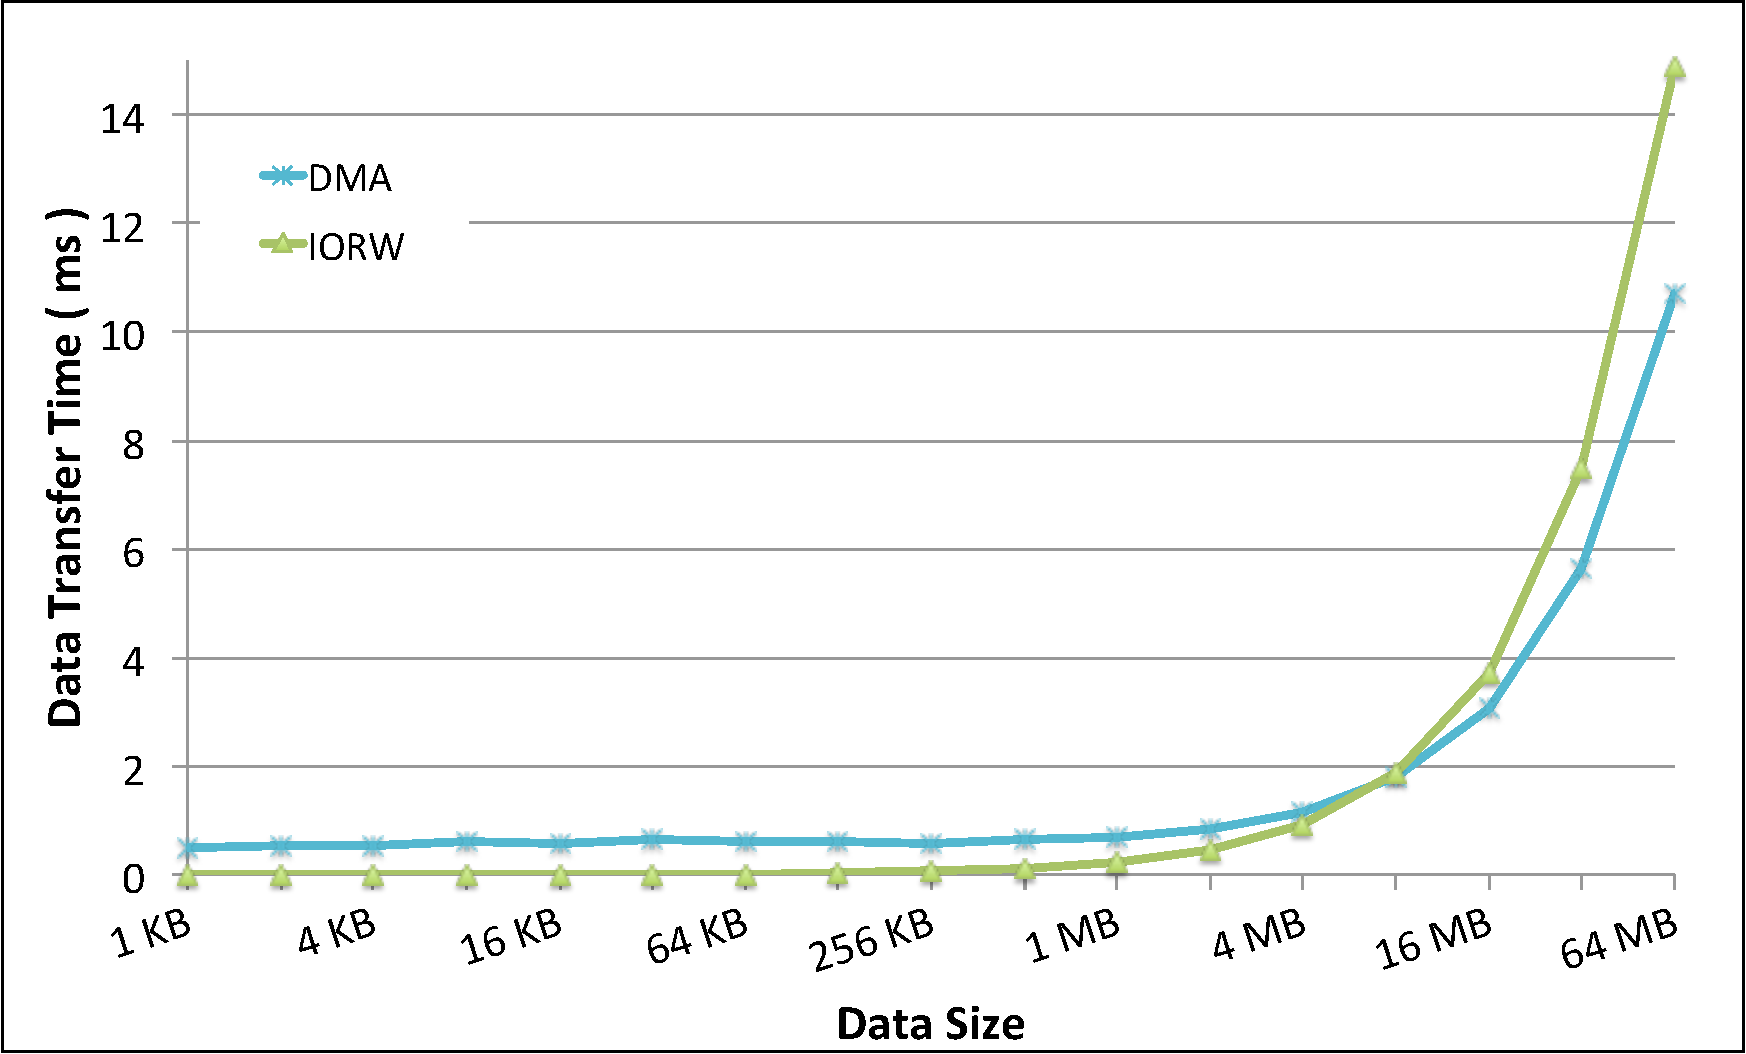
\includegraphics[width=0.34\textwidth]{figure/Graph/forIntro_HtoD.pdf}}\\
 \subfigure[Device to Host]{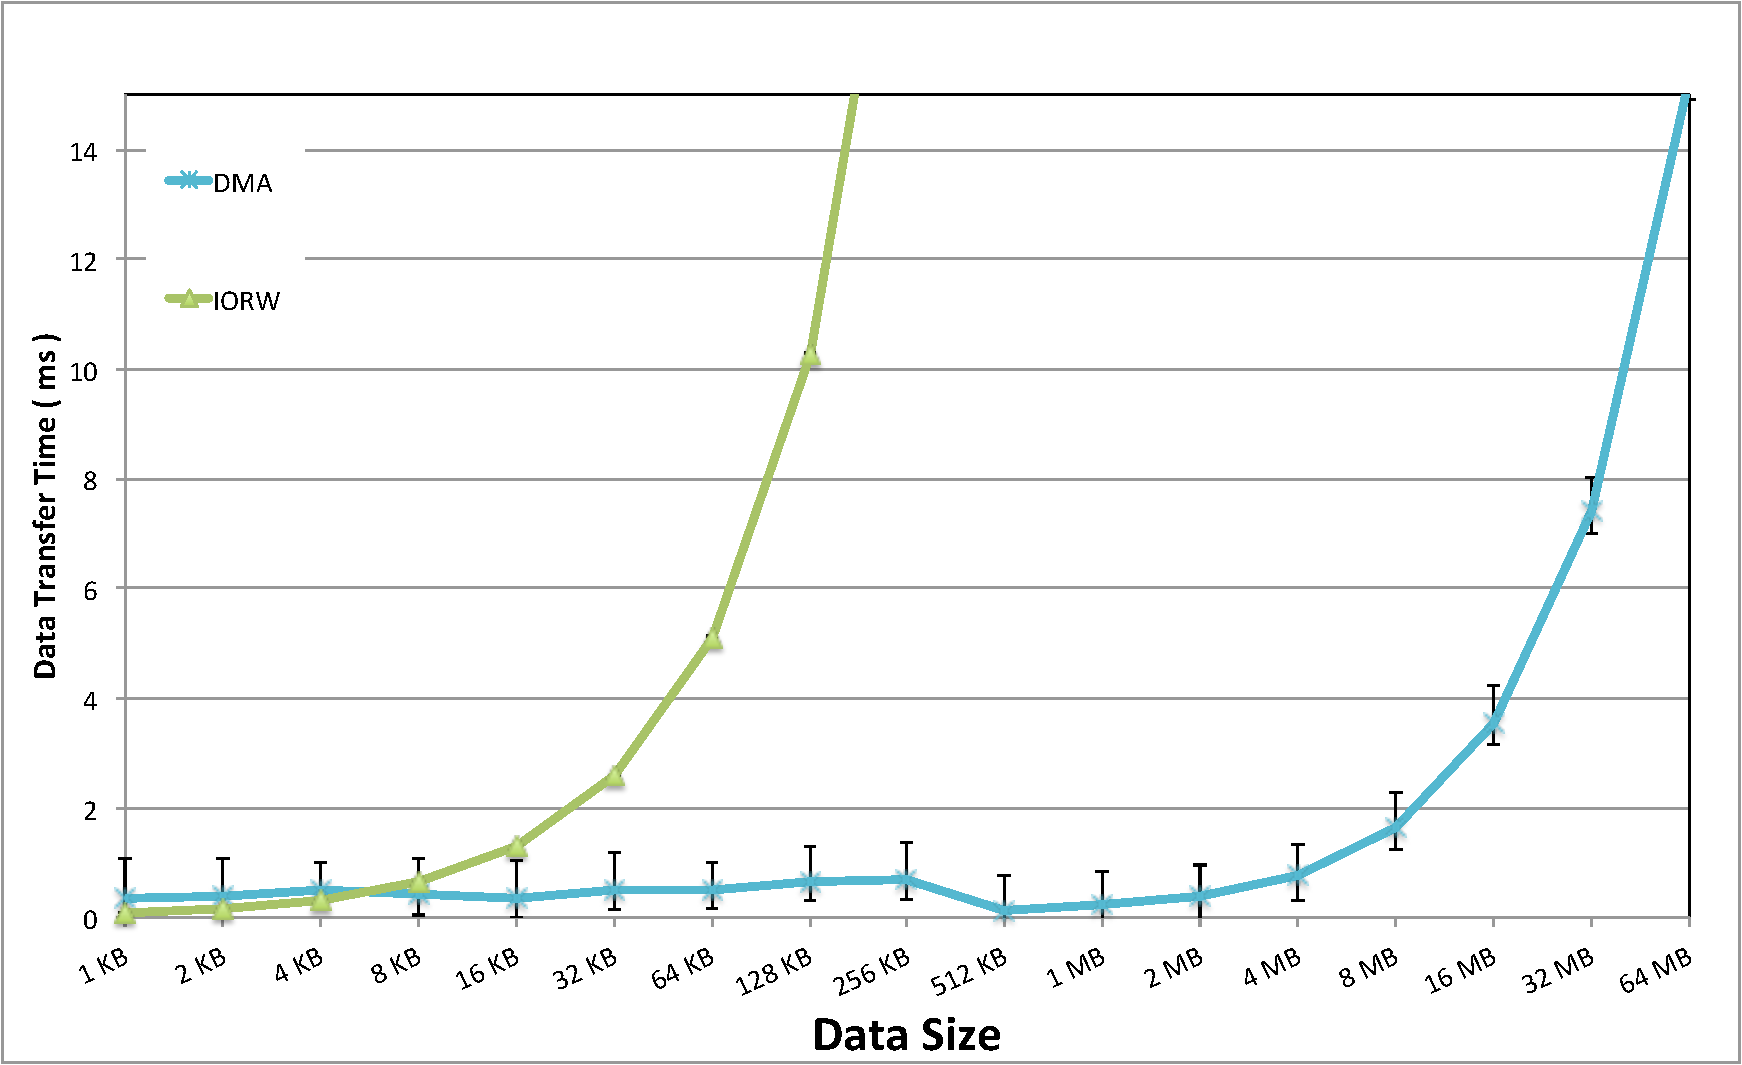
\includegraphics[width=0.34\textwidth]{figure/Graph/forIntro_DtoH.pdf}}
 \caption{Performance of DMA and I/O read/write for the GPU.}
 \label{fig:intro_data_transfer}
\end{figure}

One of the greatest challenges of GPU computing is the integration of
predictable real-time systems.
So far the real-time systems community has addressed resource management
issues of GPUs~\cite{Basaran_ECRTS12, Elliott_RTS12, Elliott_ECRTS12,
Kato_ATC11, Kato_RTAS11, Kato_RTSS11}.
The main contribution of these work is the scheduling of compute
kernels and data transfers associated with the GPU.
Given a concept of the GPU as a hardware accelerator, the basic
performance of compute kernels is not a scope of resource management
issues, but that of data transfers is managable~\cite{Kato_ATC12}.

GPU computing in the current state of the art involves many black-box
pieces.
Open-source projects have revealed key mechanisms of GPU
resource management~\cite{Kato_ATC11, Kato_ATC12}, but the hardware
details of GPUs are not disclosed to the public.
Current systems hence rely on a high-level programming framework and
limited information of proprietary sofware provided by the GPU
vendors.
This black box constraint may be acceptable for throughput-oriented
high-performane computing but 
One of the mysteries of GPU computing due to this black box constraint
is \textit{how to transfer data between the host and the device memory}.
In typical GPU-accelerated systems, the CPU executes a master flow of
the program using the host memory while the GPU executes a compute
kernel using the device memory.
This heterogeneity of GPU computing requires the program to exchange
data between the host and the device memory.
A programming framework often provides a set of data transfer methods as
part of an application programming interface (API), but their mechanisms
are encapsulated in the proprietary software implementation.

We must pray that these data transfer methods are already optimized by
the vendors.

One of the greatest challenges of GPU computing is the management of
latency issues.

nobody knows
\section{Assumption and Terminology}
\label{sec:assumption}

We assume the Compute Unified Device Architecture (CUDA) for GPU
programming~\cite{NVIDIA_CUDA}.
A unit of code that is individually launched on the GPU is called
a \textit{kernel}.
The kernel is composed of multiple \textit{threads} that execute the
code in parallel.
A unit of threads that are co-scheduled by hardware is called a
\textit{block}, while a collection of blocks for the corresponding
kernel is called a \textit{grid}.  
The maximum number of threads that can be contained by an individual
block is defined by the GPU architecture.

CUDA uses a set of an application programming interface (API) functions
to control the GPU.
A CUDA program often follows (i) allocate space
to the device memory, (ii) copy input data to the allocated device memory
space, (iii) launch the program on the GPU, (iv) copy output data back
to the host memory, and (v) free the allocated device memory space. 
The scope of this paper is related to (ii) and (iv).
In particular, we use the \texttt{cuMemCopyHtoD()} and the
\texttt{cuMemCopyDtoH()} functions of the CUDA Driver API, which
correspond to (ii) and (iv) respectively.
Since an open-source implementation of these functions is available with
Gdev~\cite{Kato_ATC12}, we modify them to accommodate the data transfer
methods investigated in this paper.

In order to focus on the performance of data transfers between the host
and the device memory, we allocate a data buffer to the pinned host
memory rather than the typical heap allocated by \texttt{malloc()}.
This pinned host memory space is mapped to the PCIe address and is never
swapped out.
It is also accessible to the GPU directly.

Our computing platform contains a single set of the CPU and the GPU.
Although we restrict our attention to CUDA and the GPU, the notion of
the investigated data transfer methods is well applicable to other
heterogeneous compute devices.
GPUs are currently well-recognized forms of the heterogeneous compute
devices, but emerging alternatives include the Intel Many Integrated
Core (MIC) and the AMD Fusion technology.
The programming models of these different platforms are almost identical
in that the CPU controls the compute devices.
Our future work includes an integrated investigation of these different
platforms.

\section{Data Transfer Methods}
\label{sec:data_transfer_methods}

In this section, we investigate data transfer methods for the GPU.
A standard data transfer method uses hardware DMA engines integrated on
the GPU, while direct data read and write accesses to the GPU device
memory are allowed through PCIe BARs.
We can also use microcontrollers integrated on the GPU to send and
receive data across the host and the device memory.
Unfortunately, only a limited piece of these schemes has been studied in
the literature.
Our investigation and open implementations of these schemes provide a
better understanding of data transfer mechanisms for the GPU.
Note that we restrict our attention to the NVIDIA GPU architecture, but
the concepts of data transfer methods introduced in this paper are
mostly applicable to PCIe-connected compute devices.

\subsection{Standard DMA}
\label{sec:dma}

\begin{figure}[!t]
 \centering
 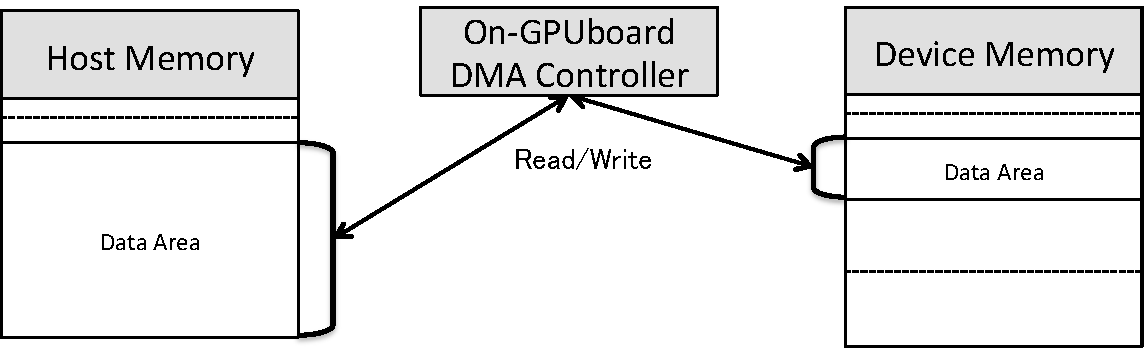
\includegraphics[width=0.45\textwidth]{figure/Method/DMA_Method.pdf}
 \caption{Standard DMA.}
 \label{fig:dma}
\end{figure}

The most typical method for GPU data transfers is to use standard DMA
engines integrated on the GPU.
There are two types of such DMA engines for synchronous and asynchronous
data transfer operations respectively.
We focus on the synchronous DMA engines, which always operate in a
sequential fashion with compute engines.

Figure~\ref{fig:dma} shows a concept of this standard DMA method.
To perform this DMA, we write \textit{GPU commands} to an on-board DMA
engine.
Upon a request of GPU commands, the DMA engine transfers a specified
data set between the host and the device memory.
Once a DMA transfer starts, it is non-preemptive.
This method is often the most effective to transfer a large size of
data.
Details of the GPU DMA mechanism can be found in previous
work~\cite{Kato_ATC11, Kato_ATC12}.

\subsection{Microcontroller-based Data Transfer}
\label{sec:micro}

\begin{figure}[!t]
 \centering
 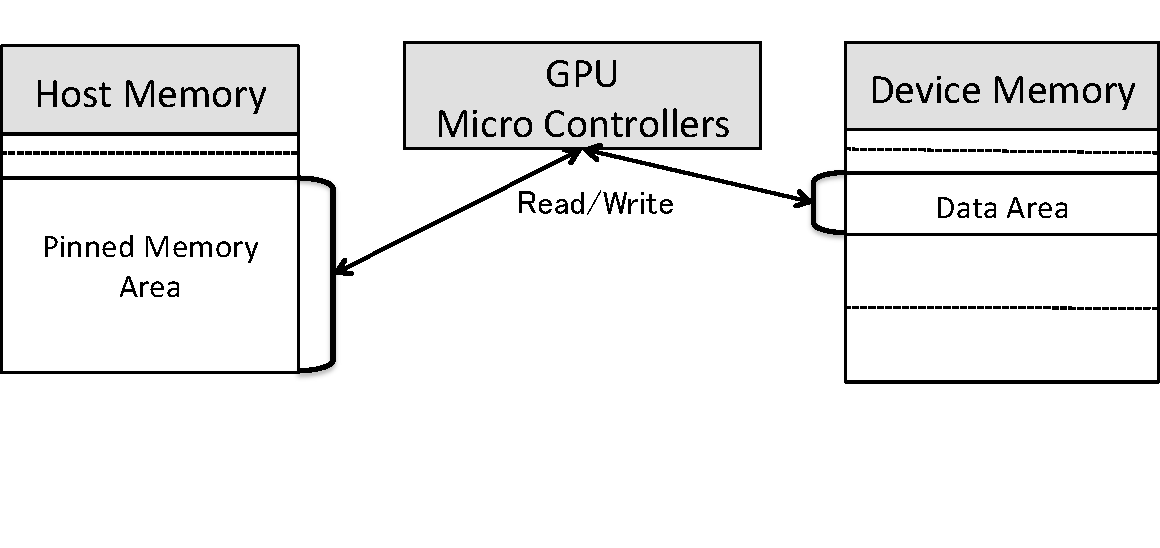
\includegraphics[width=0.45\textwidth]{figure/Method/Micro_Method.pdf}
 \caption{Microcontroller-based data transfer.}
 \label{fig:micro}
\end{figure}

The GPU provides on-board microcontrollers to control GPU functional
units (compute, DMA, power, temperature, encode, decode, etc.).
Albeit tiny hardware, these microcontrollers are available for GPU
resource management beyond just controlling the functional units.
Each microcontroller supports special instructions to transfer data in
the data sections to and from the host or the device memory.
The data transfer is offloaded to the microcontroller, \textit{i.e.},
DMA, but is controlled by the microcontroller itself.
Leveraging this mechanism, we can provide data communications between
the host and the device memory.

Figure~\ref{fig:micro} shows a concept of this microcontroller-based
data transfer method.
Since there is no data path to directly copy data between the host and
the device memory using a microcontroller, each data transfer is forced
to take two hops: (i) the host memory and microcontroller and (ii) the
device memory and microcontroller.
This is non-trivial overhead but the handling of this DMA is very
light-weight as compared to the standard DMA method.

The microcontroller is executing firmware loaded by the device driver.
We modify this firmware code to employ an interface for the data
communications.
The firmware adopts an event-driven design: it invokes only when the
device driver sends some command from the CPU.
The user program hence first needs to communicate with the device driver
to issue such a command.
Our implementation uses \texttt{ioctl} system calls to achieve this user
and device driver communication.

A constraint of this microcontroller approach is that the size of each
data transfer is limited by $256$ bytes.
If the data transfer size exceeds $256$ bytes, we have to split a
transaction into multiple chunks.

\subsection{Memory-mapped Read and Write}
\label{sec:iorw}

\begin{figure}[!t]
 \centering
 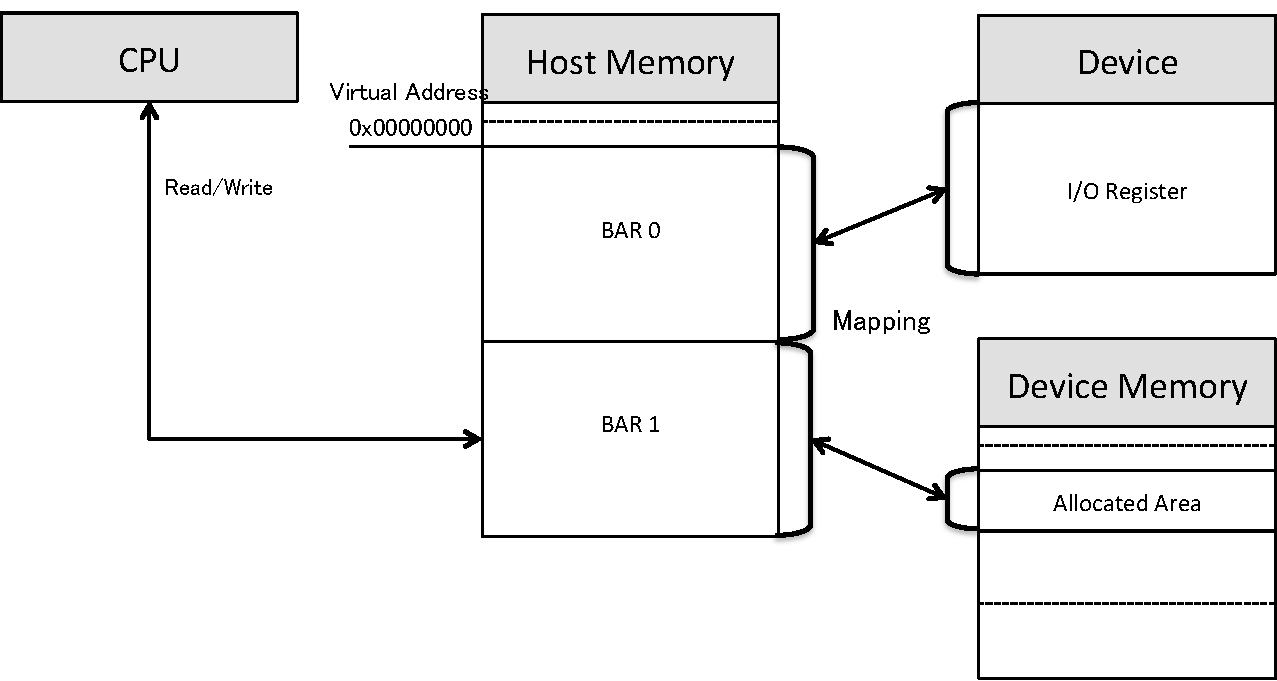
\includegraphics[width=0.45\textwidth]{figure/Method/IORW_Method.pdf}
 \caption{Memory-mapped read and write.}
 \label{fig:iorw}
\end{figure}

The aforementioned two methods are based on DMA functions.
DMA is usually high-throughput but it inevitably incurs overhead in the
setup.
A small size of data transfers may encounter severe latency problems due
to this overhead.
One of good examples can be found in the plasma control
system~\cite{Kato_ICCPS13}.
If low-latency is required, direct read and write accesses are more
appropriate than hardware-based DMA.
Since the GPU as a PCIe-connected device provides memory-mapped regions
upon the PCI address space, the CPU can directly access the device
memory without using bounce buffers on the host memory.

Figure~\ref{fig:iorw} shows a concept of this memory-mapped read and
write method.
NVIDIA GPUs as well as most other PCIe devices expose base address
registers (BARs) to the system, through which the CPU can access
specific areas of the device memory.
There are several BARs depending on the target device.
NVIDIA GPUs typically provide the following BARs:
\begin{description}
 \item[BAR0] Memory-mapped I/O (MMIO) registers.
 \item[BAR1] Device memory aperture (windows).
 \item[BAR2] I/O port or complementary space of BAR1.
 \item[BAR3] Same as BAR2.
 \item[BAR5] I/O port.
 \item[BAR6] PCI ROM.
\end{description}

Often the BAR0 is used to access the control registers of the GPU while
the BAR1 makes the device memory visible to the CPU.
This direct read and write method is pretty simple.
We create virtual address space for the BAR1 region and set its leading
address to a specific control register.
Thus the BAR1 region can be directly accessed by the GPU using the
unified memory addressing (UMA) mode, where all memory objects allocated
to the host and the device memory can be referenced by the same address
space.
Once the BAR1 region is mapped, all we have to do is to manage the page
table of the GPU to allocate memory objects from this BAR1 region and
call the I/O remapping function supported by the OS kernel to remap the
corresponding BAR1 region to the user-space buffer.

\subsection{Memory-window Read and Write}
\label{sec:memwnd}

\begin{figure}[!t]
 \centering
 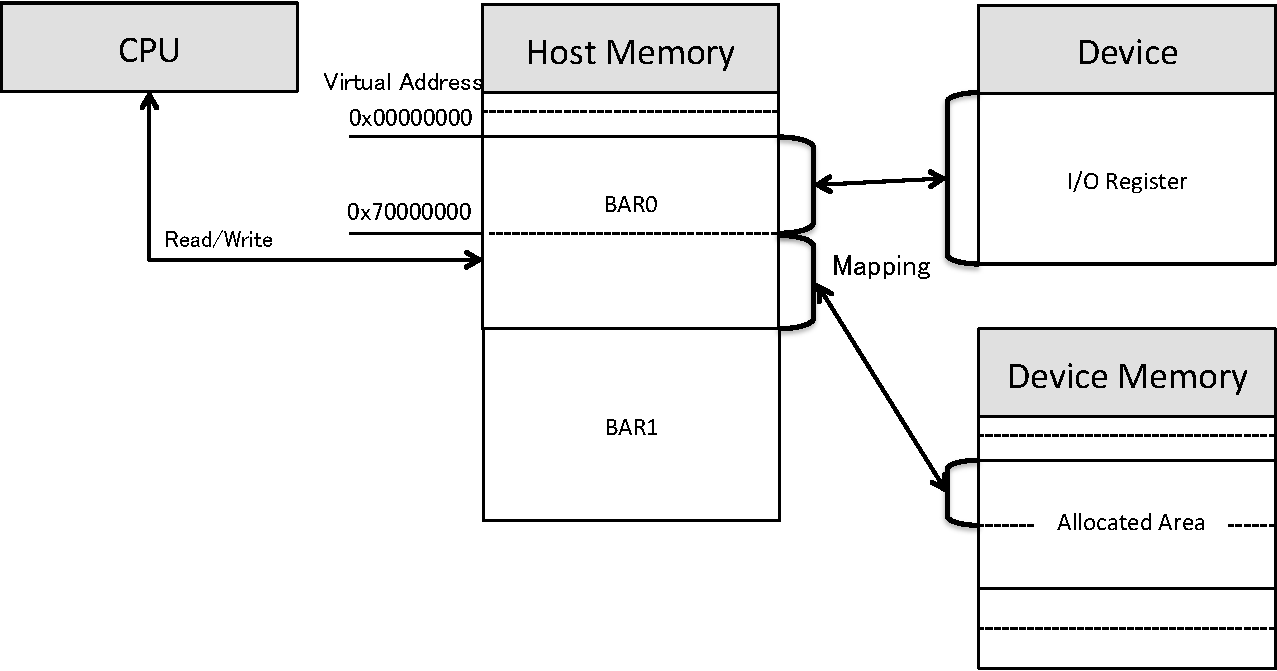
\includegraphics[width=0.45\textwidth]{figure/Method/MEMWND_Method.pdf}
 \caption{Memory-window read and write.}
 \label{fig:memwnd}
\end{figure}

The BAR0 region is often called memory-mapped I/O (MMIO) space.
This is the main control space of the GPU, through which all hardware
engines are controlled.
Its space is sparsely populated with areas representing individual
hardware engines, which in turn are sparsely populated with control
registers.
The list of hardware engines is architecture-dependent.
The MMIO space contains a special subarea for indirect device and host
memory accesses, seperated from the control registers.
This plays a role of windows that make the device memory visible to the
CPU in a different way than the BAR1 region.

Figure~\ref{fig:memwnd} shows a concept of this memory-window read and
write method.
To set the memory window, we obtain the leading physical address of the
corresponding memory object and set it to a specific control register.
By doing so, a limited range of the memory object becomes visible to the
CPU through a specific BAR0 region.
In case of NVIDIA GPUs, the size of this range is $4$MB and the specific
BAR0 region begins at 0x70000000 in the MMIO address.
Once the window is set, we can read and write this BAR0 region to access
data on the device memory.

\subsection{Pinned Host Memory}

Yet another approach to GPU data transfers is to use the pinned host
memory.
As aforementioned, NVIDIA GPUs support UMA.
This is due to the graphics address remapping table (GART) employed by
the GPU, allowing the system to specify physical host memory addresses
directly in the GPU page table as far as they are associated with pinned
PCI-mapped pages.
Although this approach is also effective to an extent for low-latency
GPU computing~\cite{Kato_ICCPS13}, it is outside the scope of this
paper and we focus on how to access the device memory in this paper.
Note that we still use the host memory as buffer space; we do not
consider a method that makes the GPU read from and write to this host
memory directly through UMA.

\section{Empirical Comparison}
\label{sec:empirical_comparison}

We now provide a detailed empirical comparison for the advantage and
disadvantage of the data transfer methods presented in
Section~\ref{sec:data_transfer_methods}.
Our experimental setup is composed of an Intel Core i7 2600 processor
and an NVIDIA GeForce GTX~480 graphics card.
We use the Linux kernel v2.6.42 and Gdev~\cite{Kato_ATC12} as the
underlying OS and GPGPU runtime/driver software respectively.
This set of open-source platforms allows our implementations of the
investigated data transfer methods.

The test programs are written in CUDA~\cite{NVIDIA_CUDA} and are compiled
using the NVIDIA CUDA Compiler (NVCC) v4.2~\cite{NVIDIA_NVCC}.
Note that Gdev is compatible with this binary compiler toolkit.
We exclude compute kernels and focus on data transfer functions in this
empirical comparison.
While the test programs uniformly use the same CUDA API functions, we
provide different internal implementations according to the target data
transfer methods.

Data streams between the host and the device memory are provided by a
single GPU context.
Performance interference among multiple GPU contexts is outside the
scope of this paper.
We evaluate the data transfer performances of both real-time and normal
tasks.
For the scheduling policies of the Linux kernel, we use
\texttt{SCHED\_FIFO} for real-time tasks while \texttt{SCHED\_OTHER} for
normal tasks, where the real-time tasks are always prioritized over the
normal tasks.
The real-time capability relies on the default performance of the
real-time scheduling class supported by the Linux kernel.
We believe that this setup is sufficient for our experiments given that
we execute at most one real-time task in the system while multiple data
streams may be produced by this task.
Overall the scheduling performance issues are outside the scope of this
paper.

Henceforth we use the following labels to denote the investigated data
transfer methods respectively:
\begin{itemize}
 \item \textbf{DMA} denotes the standard DMA method presented in
       Section~\ref{sec:dma}.
 \item \textbf{IORW} denotes the memory-mapped read and write method
       presented in Section~\ref{sec:iorw}.
 \item \textbf{MEMWND} denotes the memory-window read and write method
       presented in Section~\ref{sec:memwnd}.
 \item \textbf{HUB} denotes the microcontroller-based data transfer
       method presented in Section~\ref{sec:micro}, particularly using a
       \textit{hub} microcontroller designed to broadcast among the
       actual microcontrollers of graphics processing clusters (GPCs),
       \textit{i.e.}, CUDA core clusters.
 \item \textbf{GPC} denotes the microcontroller-based data transfer
       method presented in Section~\ref{sec:micro}, particularly using a
       single GPC microcontroller.
 \item \textbf{GPC4} denotes the microcontroller-based data transfer
       method presented in Section~\ref{sec:micro}, particularly using
       four different GPC microcontrollers in parallel.
       Note that the NVIDIA Fermi architecture~\cite{NVIDIA_Fermi}
       provides four GPCs and their microcontrollers can perform
       individually.
       Therefore we can split the data transfer into four pieces and
       make the four microcontrollers work in parallel.
\end{itemize}

\subsection{Basic Performance}
\label{sec:basic_performance}

\begin{figure}[!t]
 \begin{center}
  \subfigure[Host to Device]{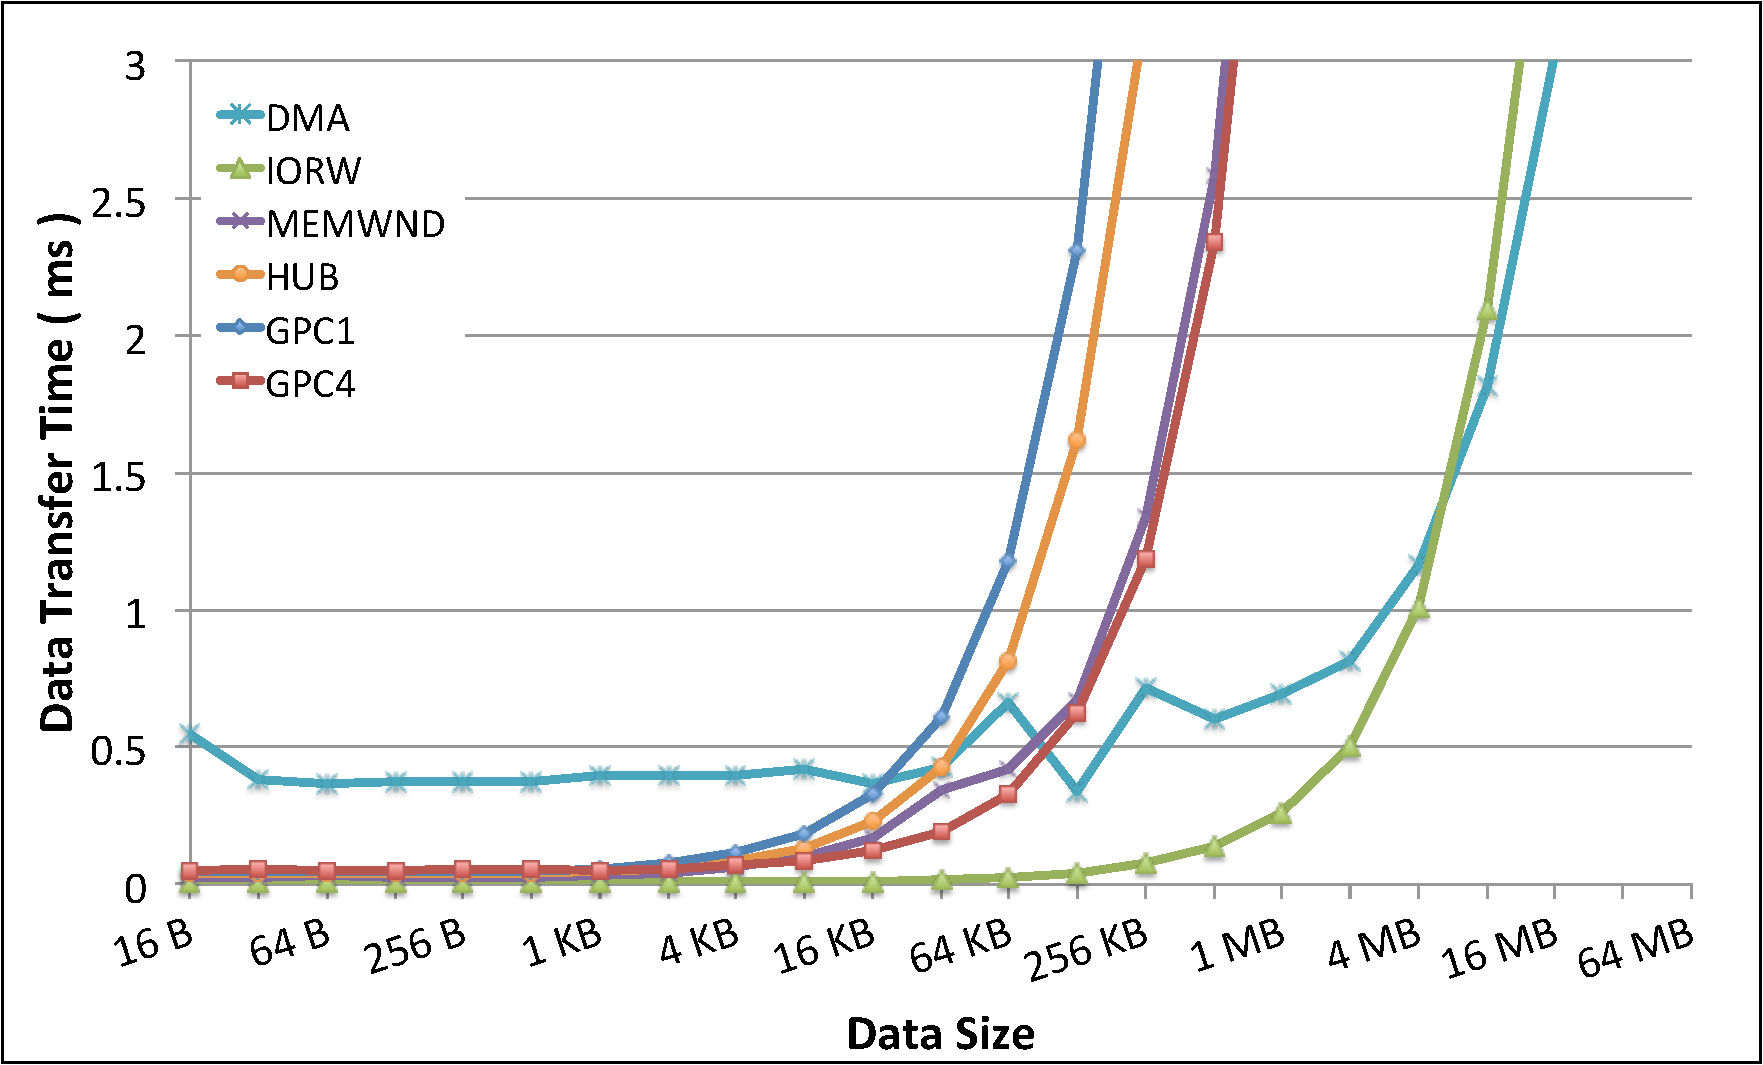
\includegraphics[width=0.34\textwidth]{figure/Graph/realtask/Memcpy_rtask_normal_HtoD.pdf}}\\
  \subfigure[Device to Host]{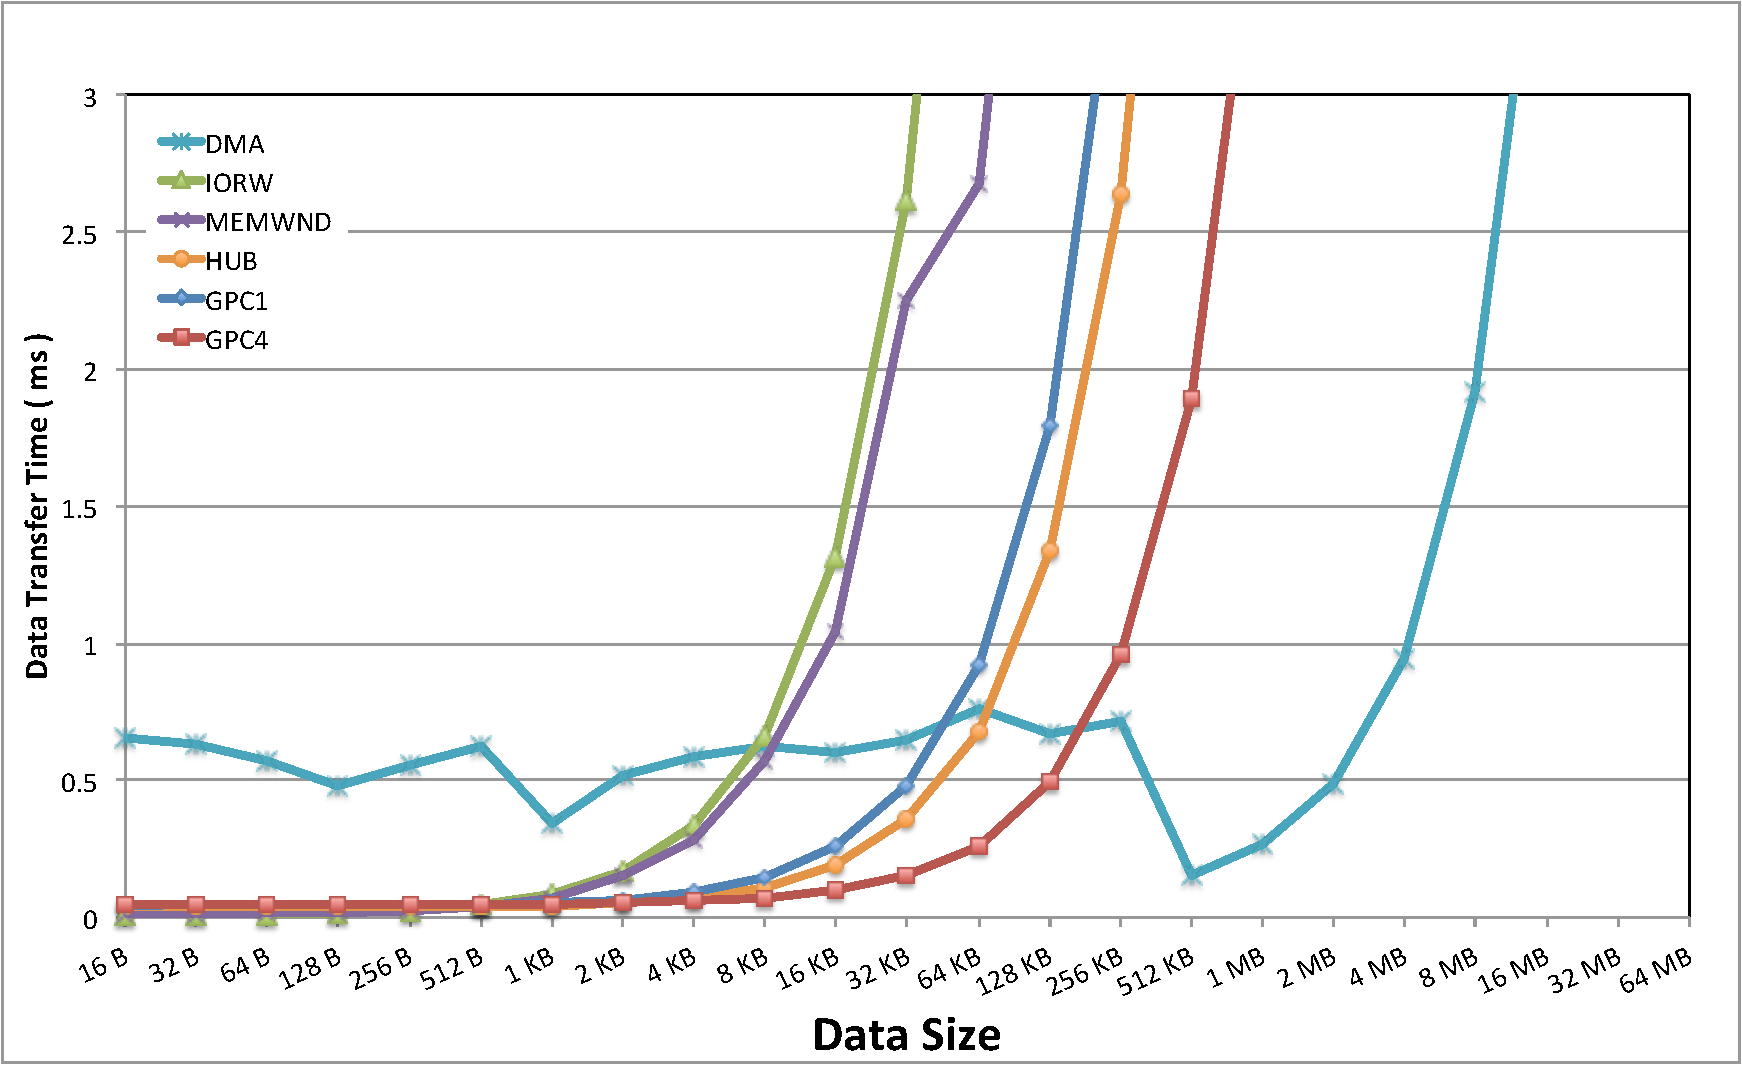
\includegraphics[width=0.34\textwidth]{figure/Graph/realtask/Memcpy_rtask_normal_DtoH.pdf}}
  \caption{Average performance of each data transfer method with a
  real-time task.}
  \label{fig:average_realtime}
 \end{center}
\end{figure}
\begin{figure}[!t]
 \begin{center}
  \subfigure[Host to Device]{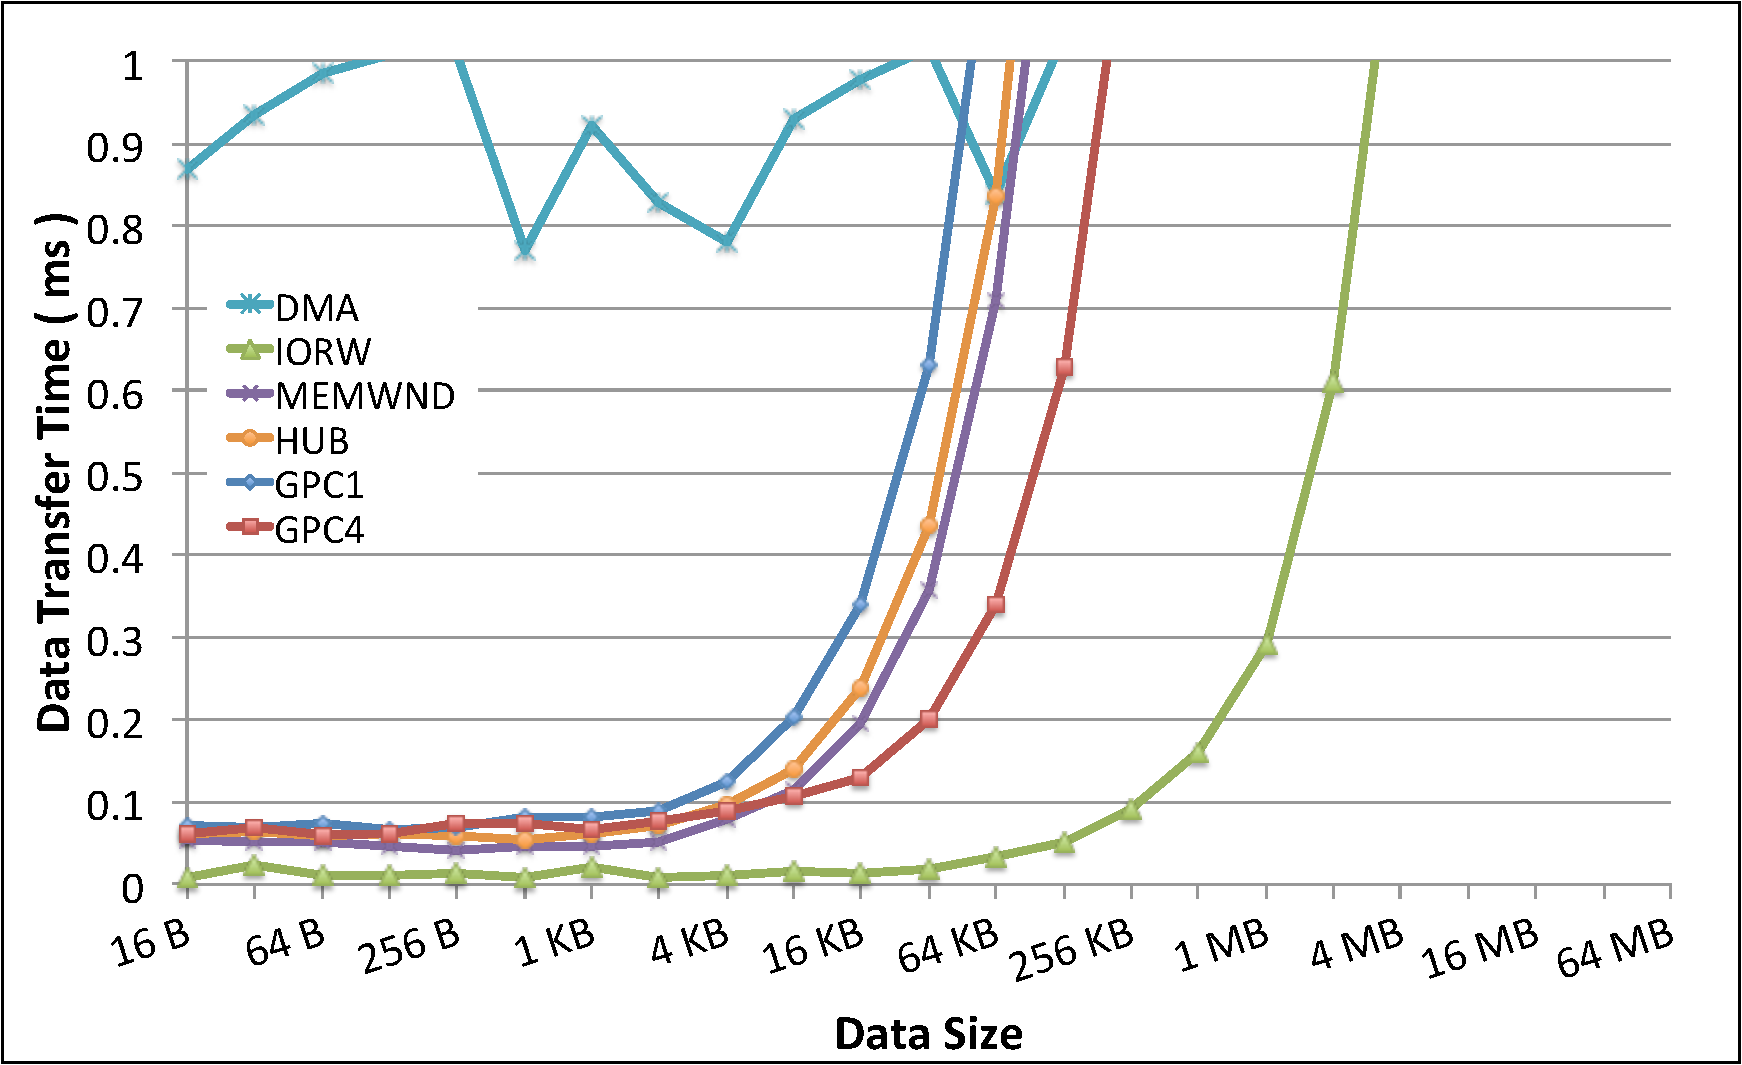
\includegraphics[width=0.34\textwidth]{figure/Graph/realtask/Memcpy_rtask_normal_HtoD_worst.pdf}}\\
  \subfigure[Device to Host]{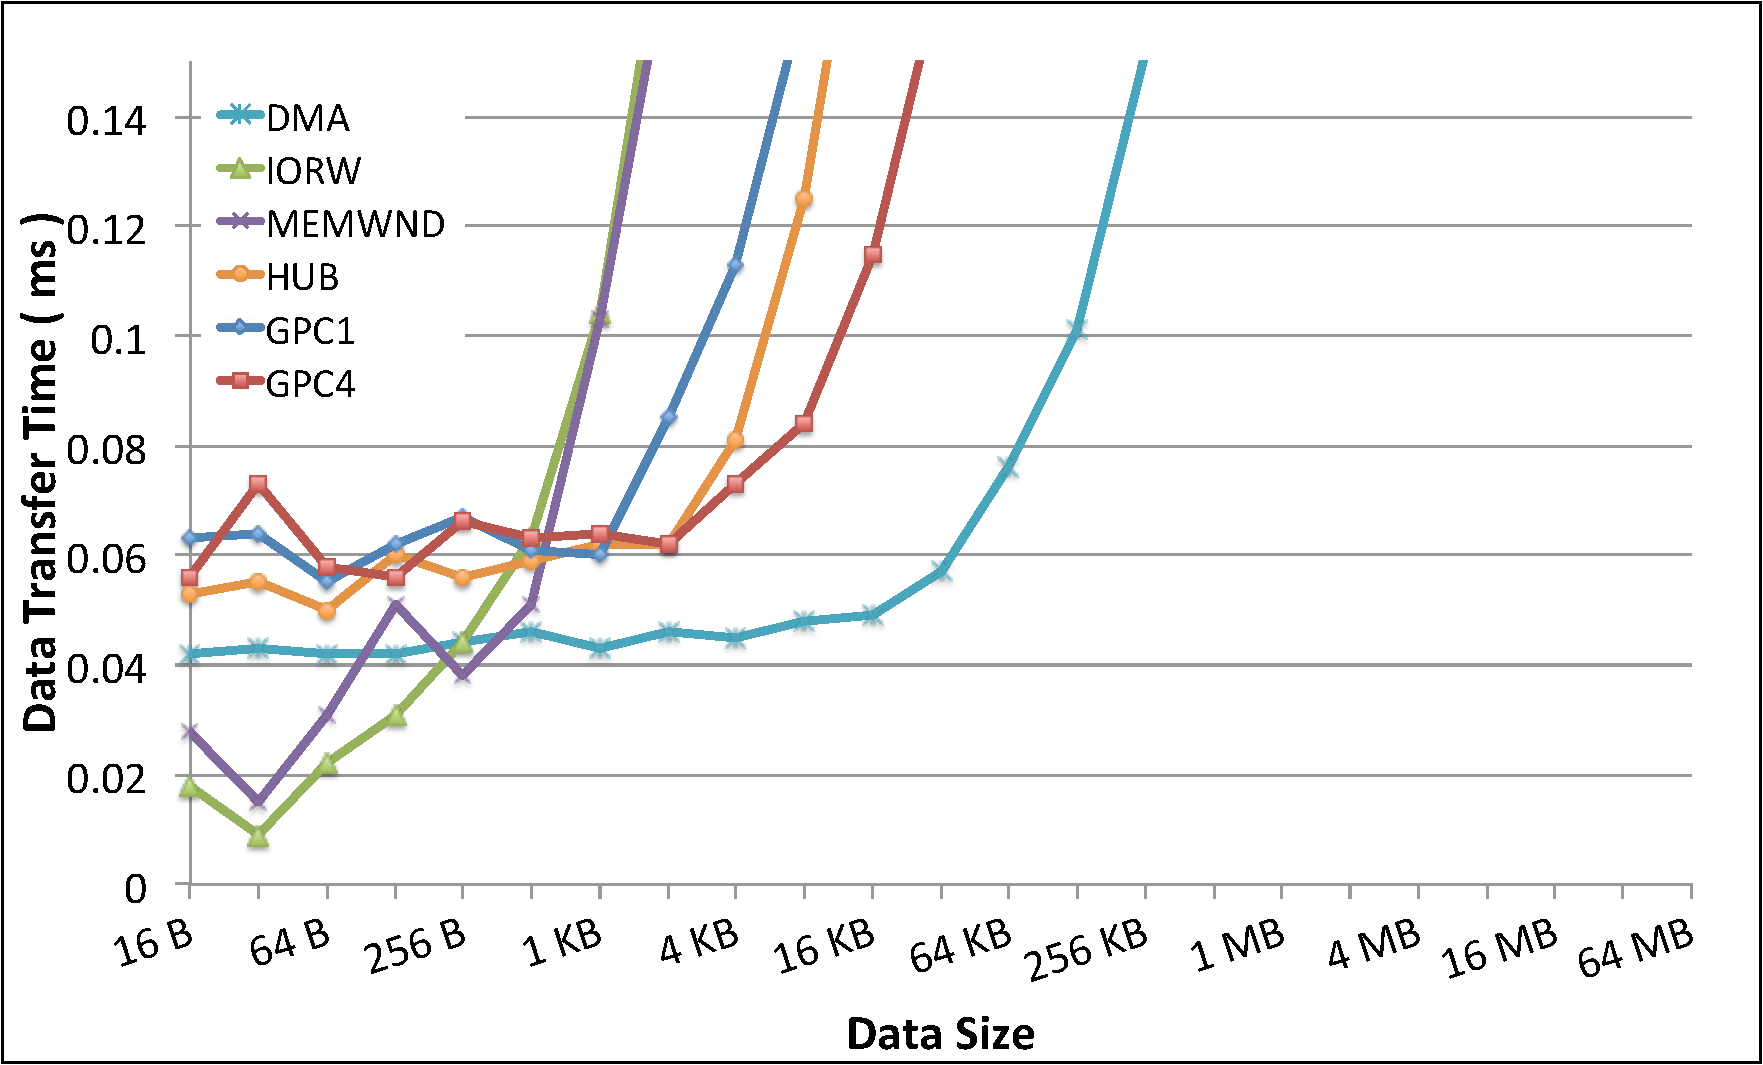
\includegraphics[width=0.34\textwidth]{figure/Graph/realtask/Memcpy_rtask_normal_DtoH_worst.pdf}}
  \caption{Worst-case performance of each data transfer method with a
  real-time task.}
  \label{fig:worst_realtime}
 \end{center}
\end{figure}

Figure~\ref{fig:average_realtime} shows the average performance of each
data transfer method when a real-time task runs alone.
Even with this most straightforward setup, there are several interesting
observations.
Performance characteristics of the host-to-device and the device-to-host
communications are not identical at all.
In particular the performance of standard DMA exhibits a 10x difference
between the two directions of communications.
We believe that this is due to hardware capabilities that are not
documented to the public.
We also find that the performances of different methods are diverse but
either \textsf{DMA} or \textsf{IORW} can derive the best performance for
any data size.
In case of the host-to-device direction, for small data from $16$B to
$8$MB, \textsf{IORW} is preferred, while \textsf{DMA} outperforms
\textsf{IORW} larger data than $8$MB.
The other methods are almost always inferior to either of \textsf{DMA}
or \textsf{IORW}.
The most significant finding is that \textsf{IORW} becomes very slow for
the device-to-host direction.
It is faster than \textsf{DMA} only until $512$B.
This is due to a design specification of the GPU.
It is designed so that the GPU can read data fast from the host computer
but compromise write access performance.
Another interesting observation is that using multiple GPC
microcontrollers to parallelize the data transfer is less effective than
a single GPC or HUB controller when the data size is small.

Figure~\ref{fig:worst_realtime} shows the worst-case performance in
the same setup as the above experiment.
It is important to note that we acquire almost the same results as those
shown in Figure~\ref{fig:average_realtime}, though there is
some degradation in the performance of \textsf{DMA} for the
host-to-device direction.
These comparisons lead to some conclusion that we may optimize the data
transfer performance by switching between \textsf{DMA} and \textsf{IORW}
at an appropriate boundary.

We omit the results of normal tasks in this setup, because they are
almost equal to those of real-time tasks shown above.
However, real-time and normal tasks behave in a very different manner in
the presence of competing workload.
This will be discussed in the next subsection.

\subsection{Interfered Performance}
\label{sec:interfered_performance}

\begin{figure}[!t]
 \begin{center}
  \subfigure[Host to Device]{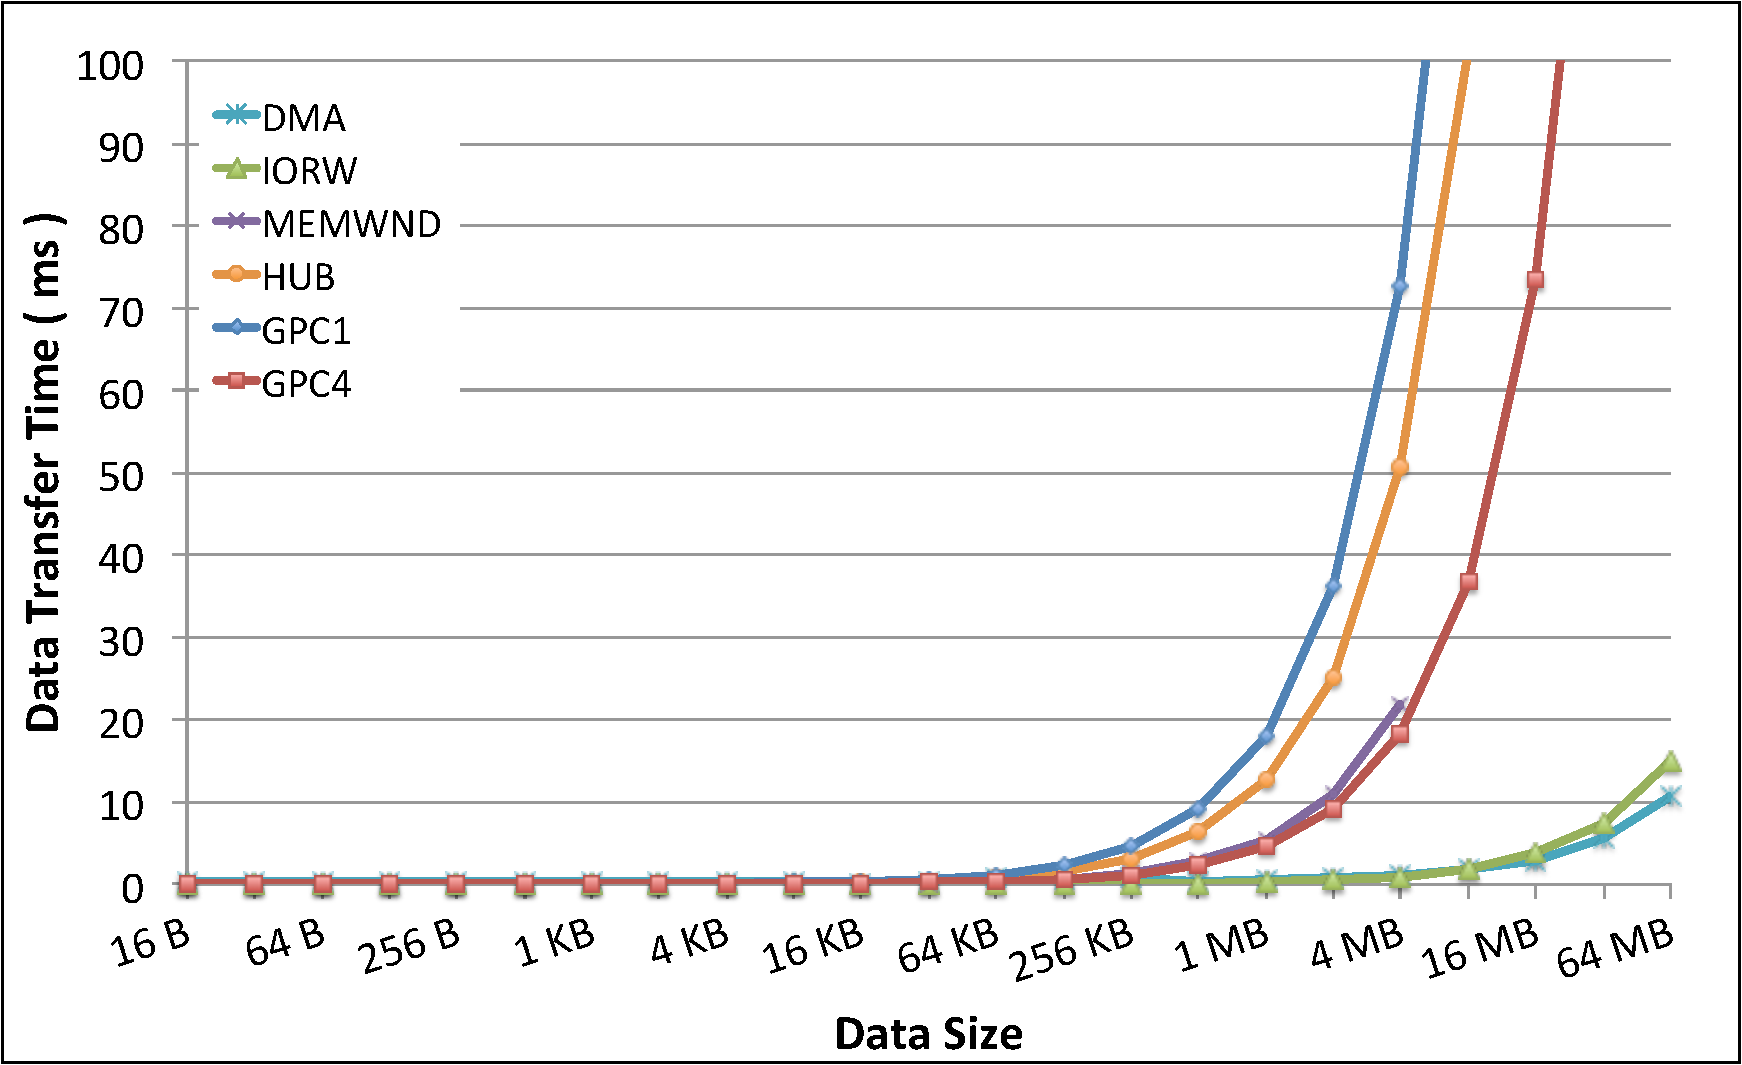
\includegraphics[width=0.34\textwidth]{figure/Graph/realtask/Memcpy_rtask_cpuload_HtoD.pdf}}\\
  \subfigure[Device to Host]{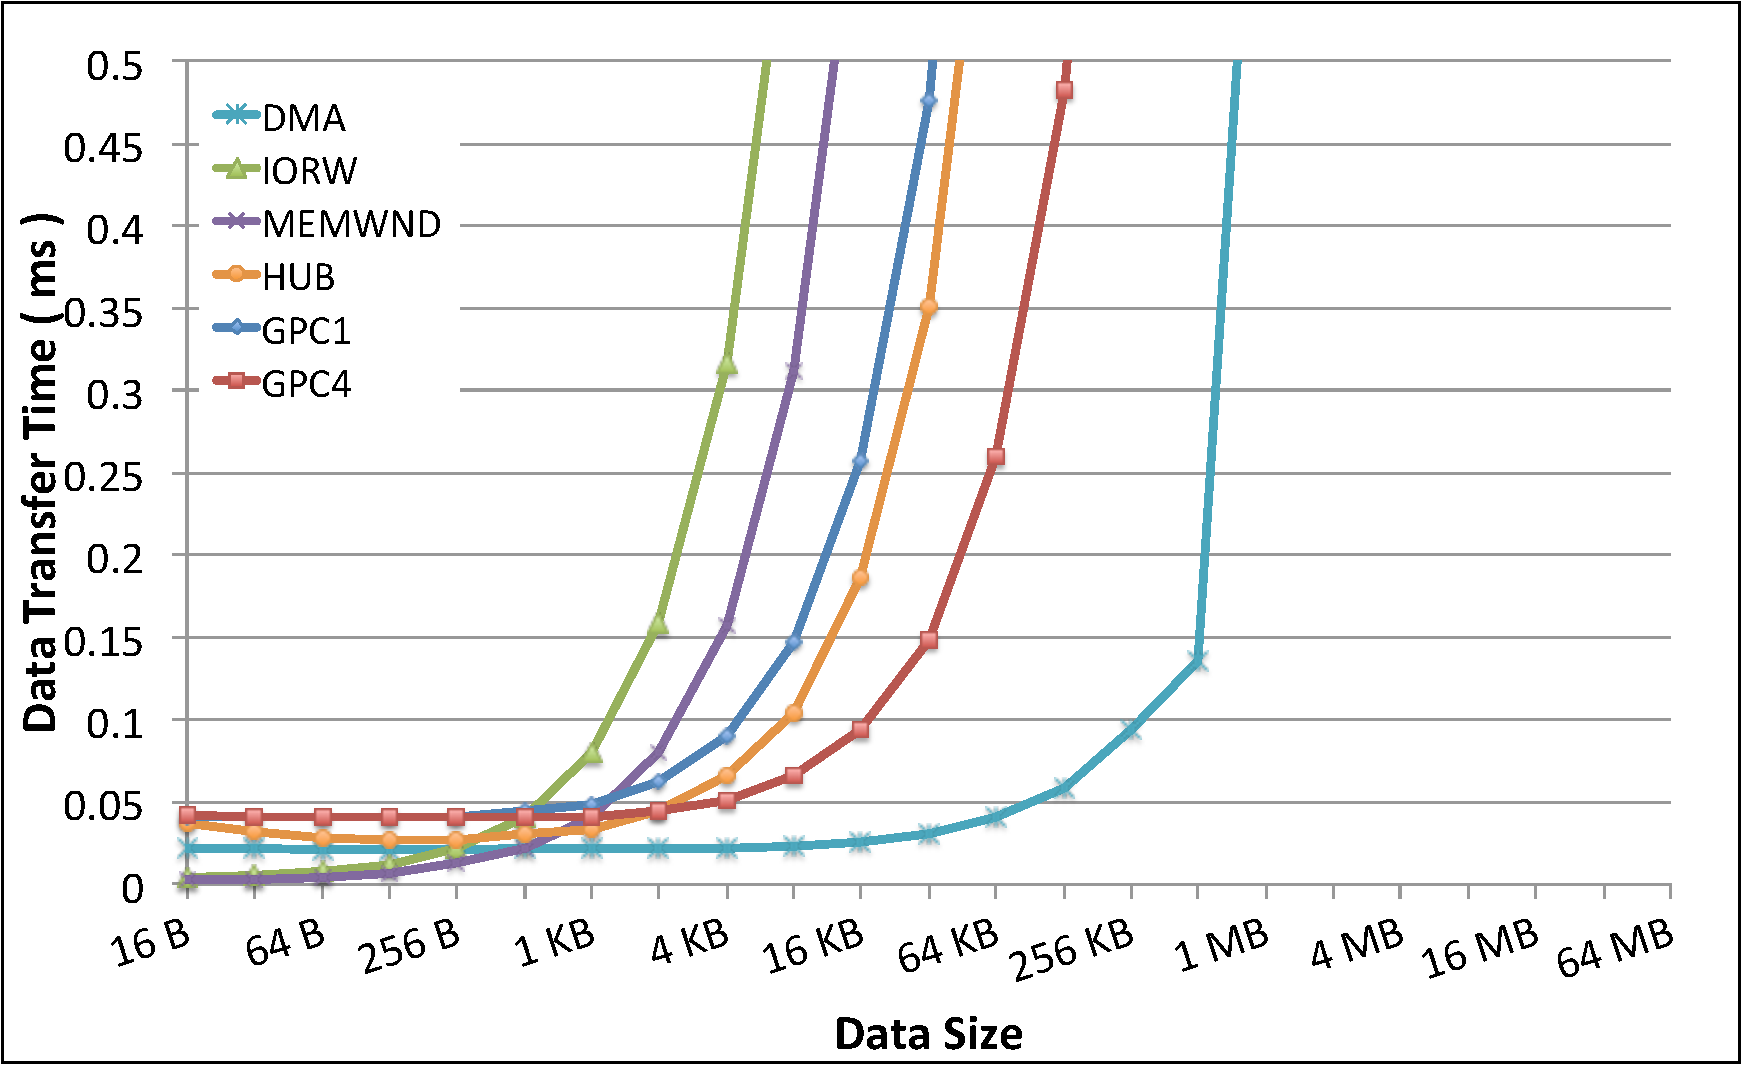
\includegraphics[width=0.34\textwidth]{figure/Graph/realtask/Memcpy_rtask_cpuload_DtoH.pdf}}
  \caption{Average performance of each data transfer method with a
  real-time task under high CPU load.}
  \label{fig:average_realtime_cpuload}
 \end{center}
\end{figure}
\begin{figure}[!t]
 \begin{center}
  \subfigure[Host to Device]{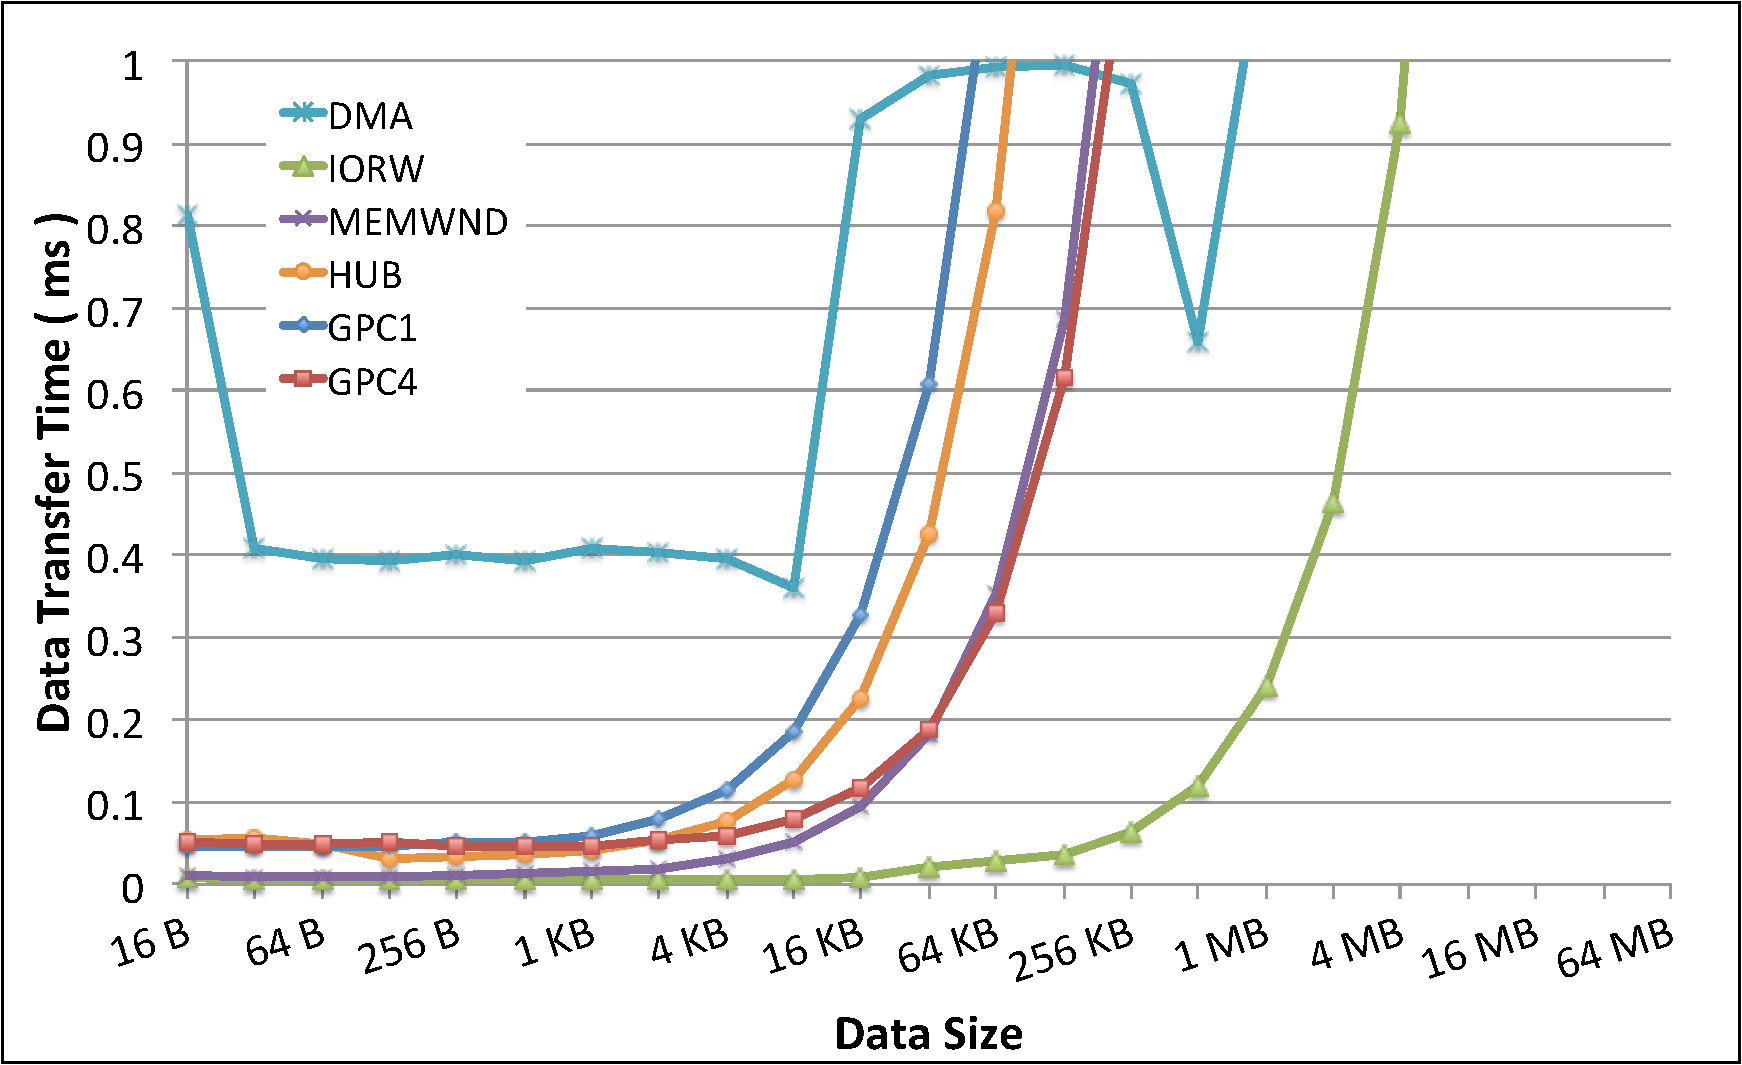
\includegraphics[width=0.34\textwidth]{figure/Graph/realtask/Memcpy_rtask_cpuload_HtoD_worst.pdf}}\\
  \subfigure[Device to Host]{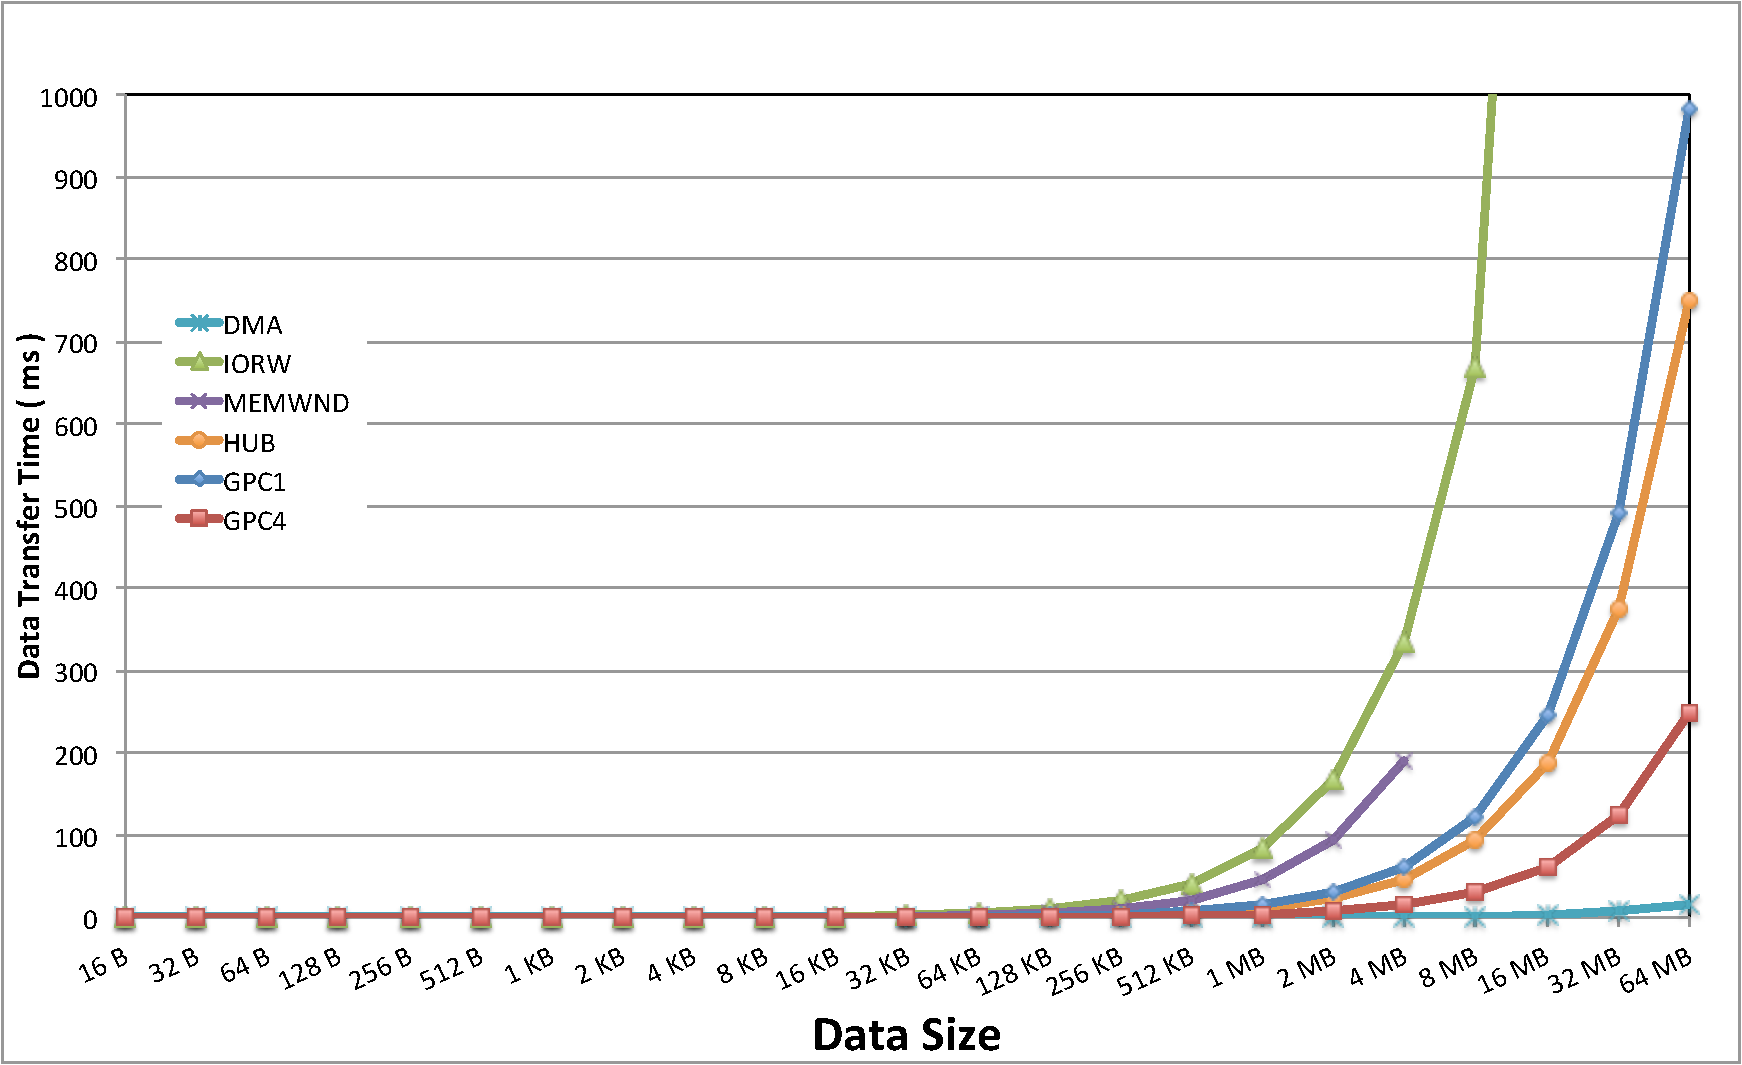
\includegraphics[width=0.34\textwidth]{figure/Graph/realtask/Memcpy_rtask_cpuload_DtoH_worst.pdf}}
  \caption{Worst-case performance of each data transfer methods with a
  real-time task under high CPU load.}
  \label{fig:worst_realtime_cpuload}
  \end{center}
\end{figure}

Figure~\ref{fig:average_realtime_cpuload} shows the average performance
of each data transfer method when a real-time task encounters extremely
high workload on the CPU.
All the methods are successfully protected from performance interference
due to the real-time scheduler.
Note that \textsf{DMA} shows a better performance than the previous
experiments despite the presence of competing workload.
This is due to the Linux real-time scheduler feature.
\textsf{DMA} is performed by GPU commands, which may impose a
suspension on the caller task.
In the Linux kernel, a real-time task is awakened in a more responsive
manner when switched from a normal task than from an idle task.
Therefore when the CPU is fully loaded by normal tasks, a real-time task
is more responsive.
The same is true for the worst-case performance as shown in
Figure~\ref{fig:worst_realtime_cpuload}.
We learn from these experiments that CPU priorities can protect the
performance of data transfer for the GPU.
Note that Gdev uses a polling approach to wait for completions of data
transfers.
An interrupt approach is also worth being investigated.

\begin{figure}[!t]
 \begin{center}
  \subfigure[Host to Device]{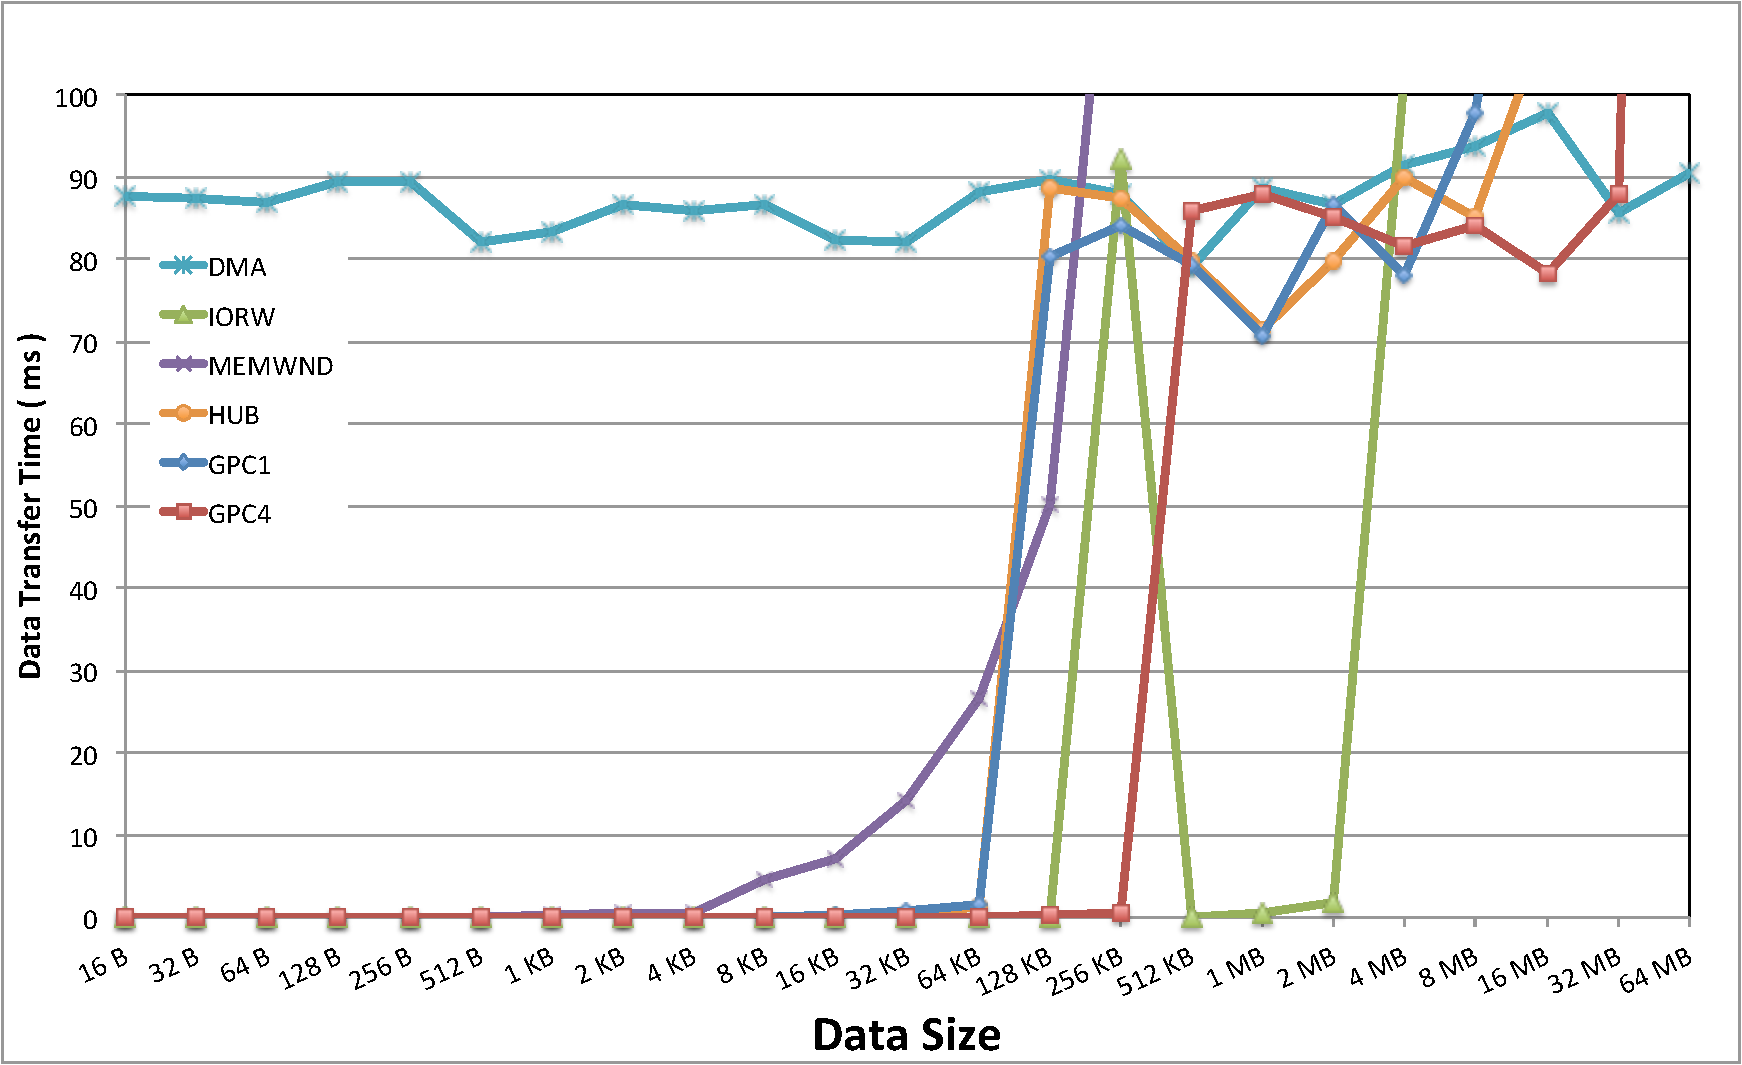
\includegraphics[width=0.34\textwidth]{figure/Graph/not_realtask/Memcpy_cpuload_HtoD.pdf}}\\
  \subfigure[Device to Host]{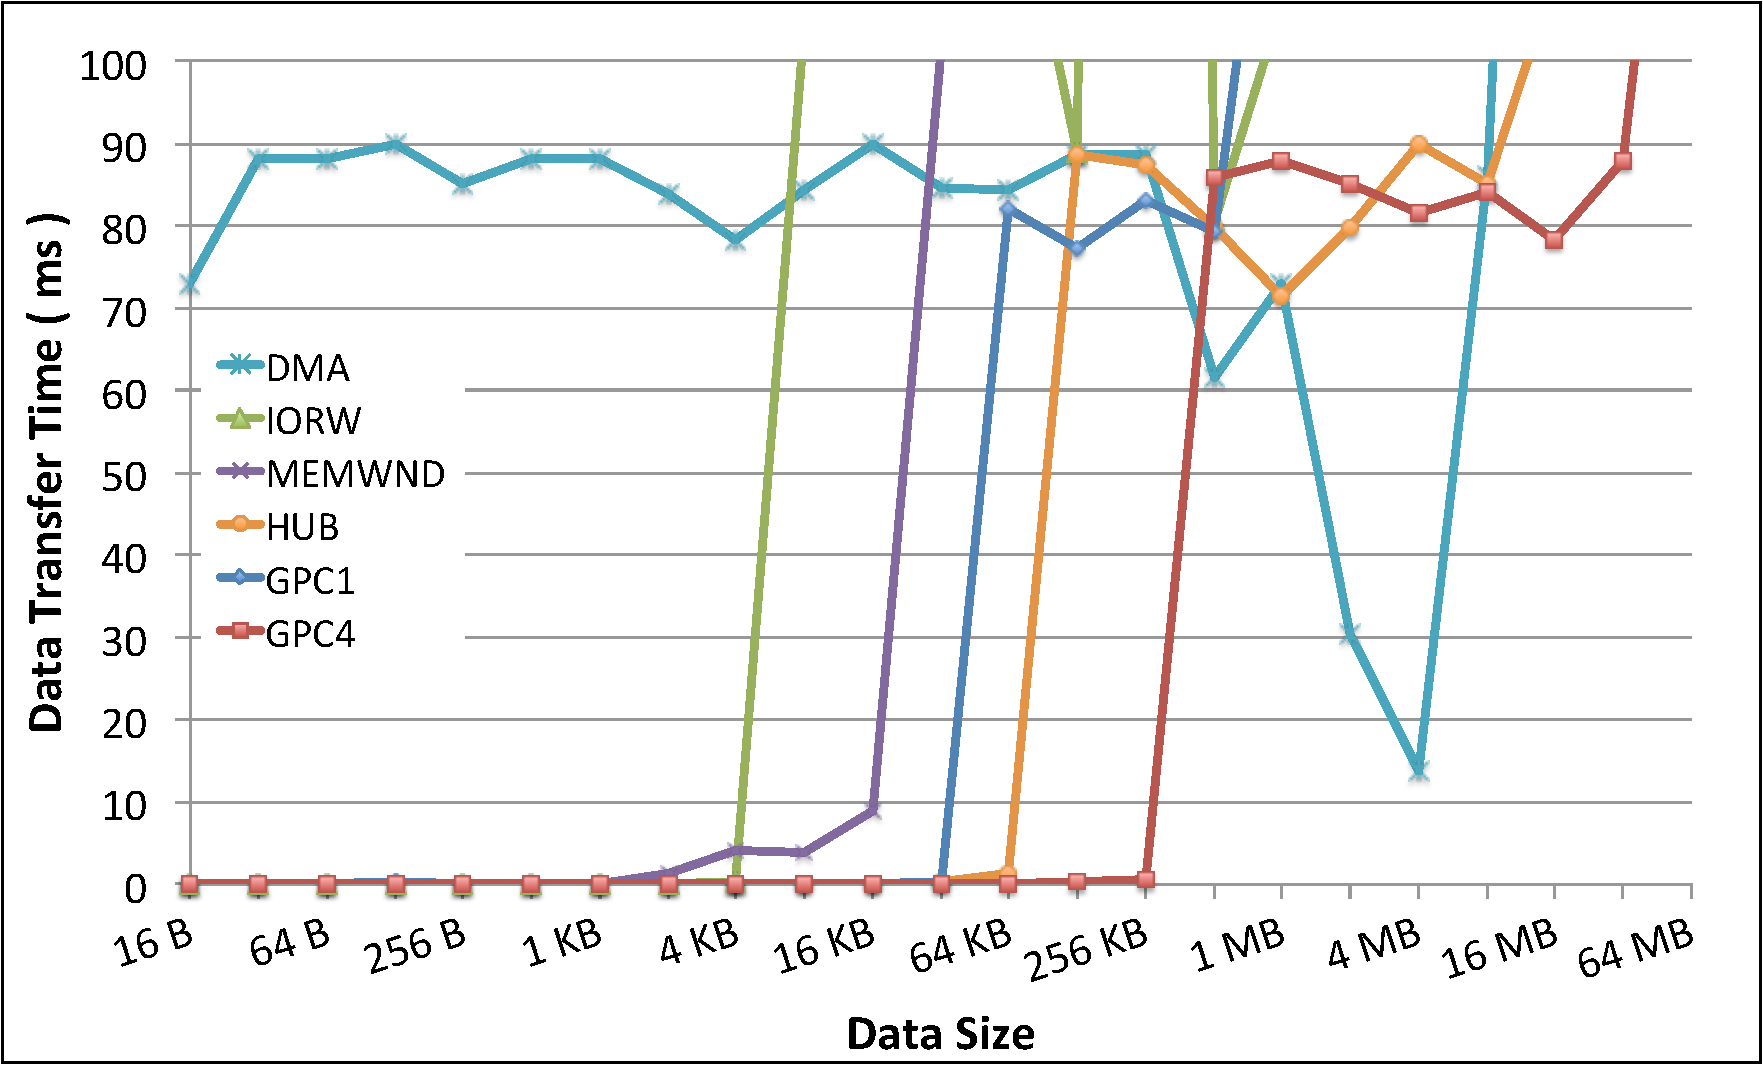
\includegraphics[width=0.34\textwidth]{figure/Graph/not_realtask/Memcpy_cpuload_DtoH.pdf}}
  \caption{Average performance of each data transfer method with a
  normal data stream under high CPU load.}
  \label{fig:average_normal_cpuload}
 \end{center}
\end{figure}
\begin{figure}[!t]
 \begin{center}
  \subfigure[Host to Device]{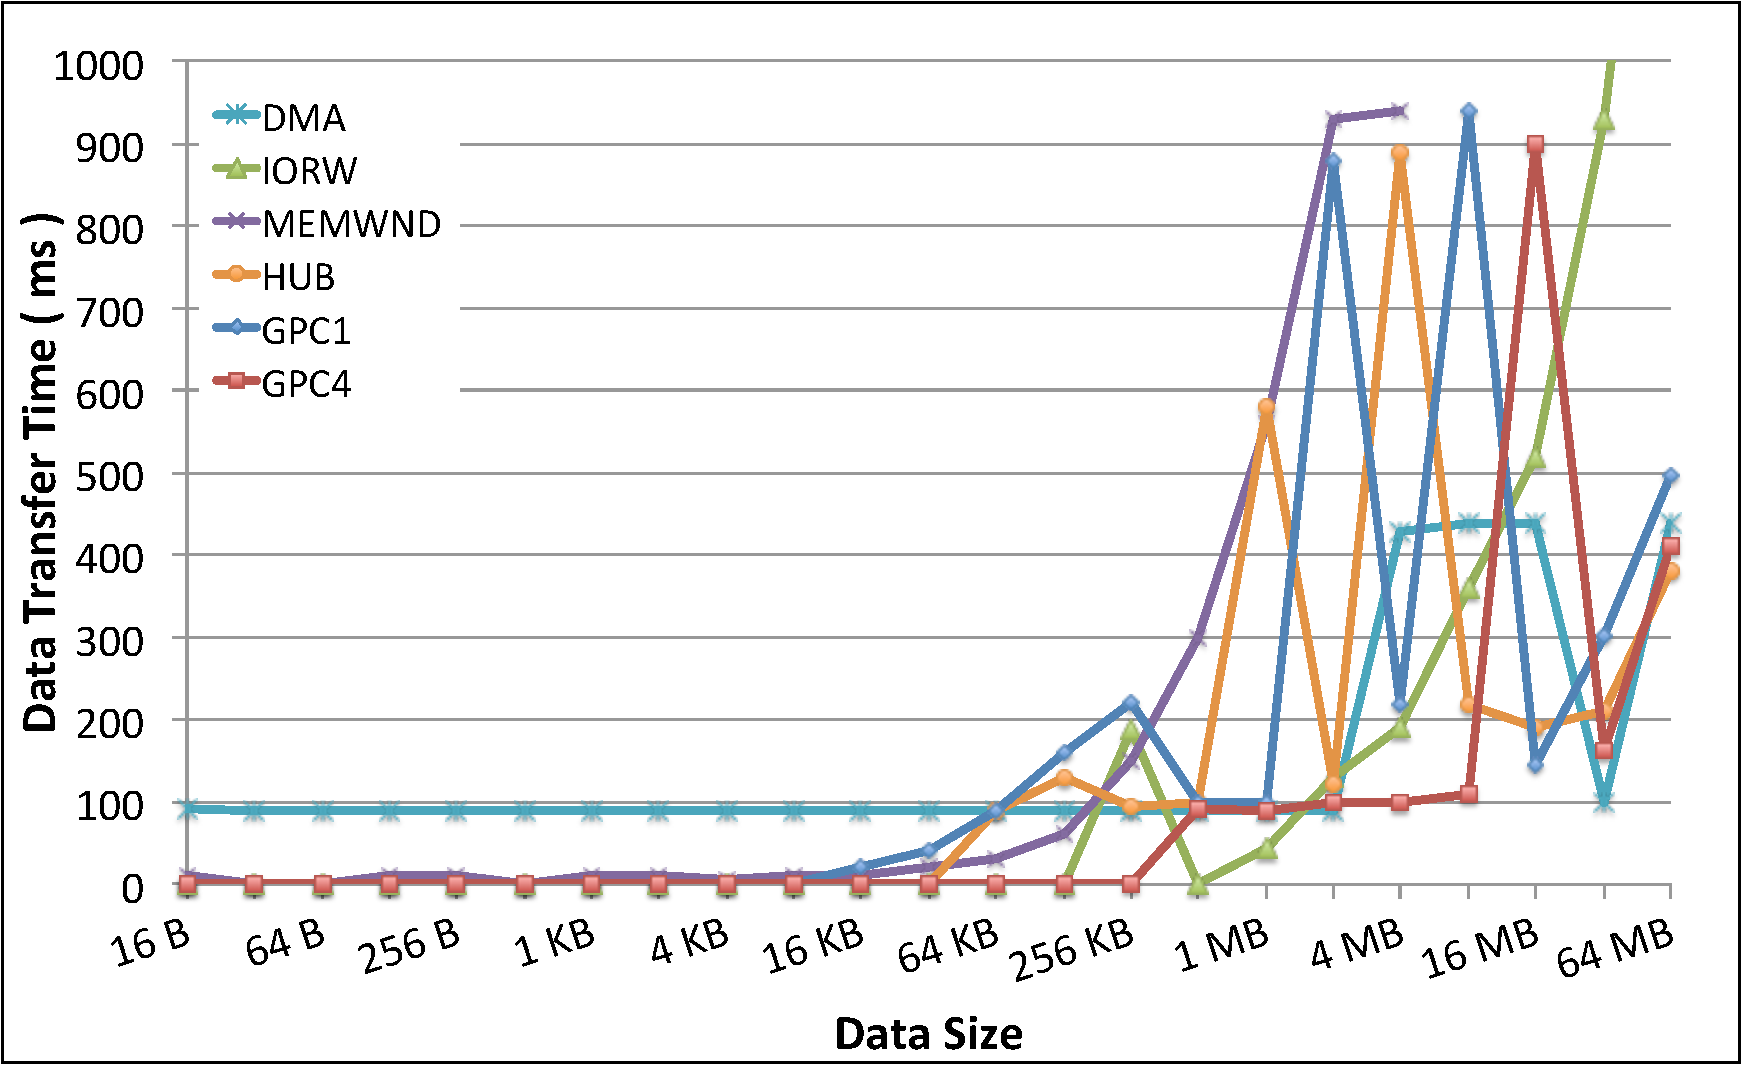
\includegraphics[width=0.34\textwidth]{figure/Graph/not_realtask/Memcpy_cpuload_HtoD_worst.pdf}}\\
  \subfigure[Device to Host]{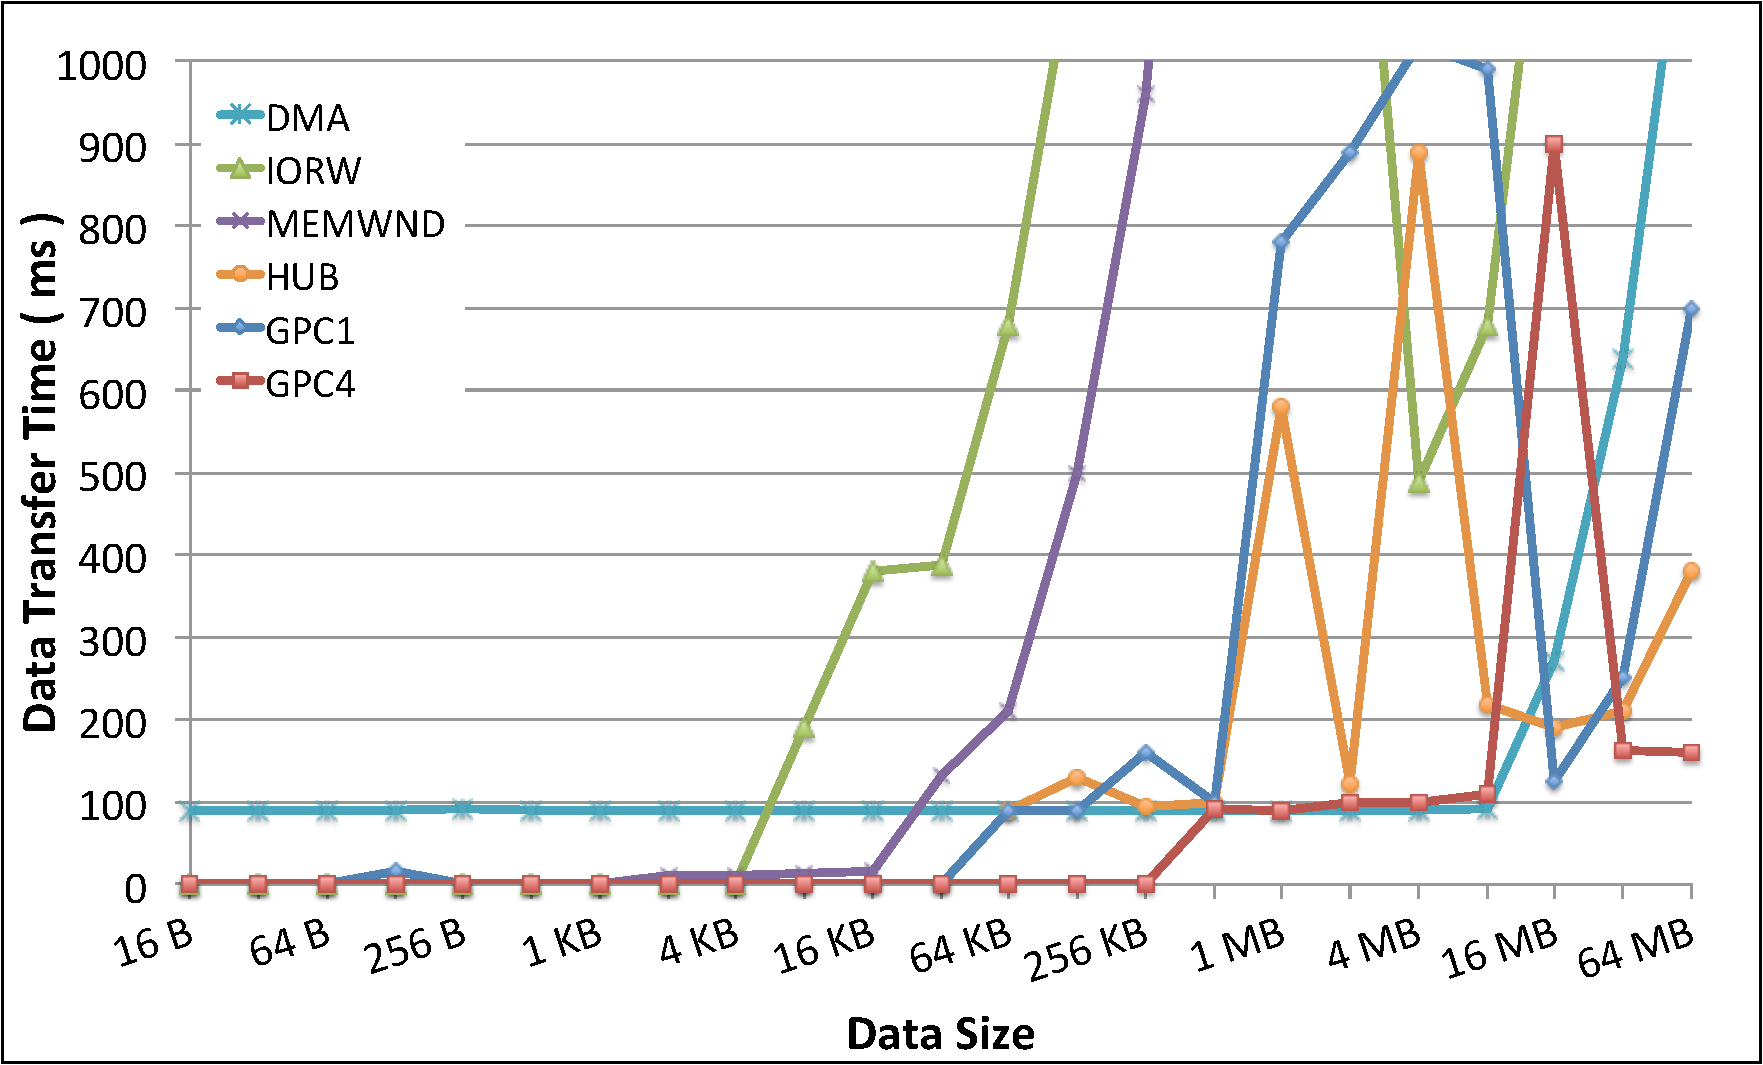
\includegraphics[width=0.34\textwidth]{figure/Graph/not_realtask/Memcpy_cpuload_DtoH_worst.pdf}}
  \caption{Worst-case performance of each data transfer method with a
  normal data stream under high CPU load.}
  \label{fig:worst_normal_cpuload}
 \end{center}
\end{figure}

For reference,
Figure~\ref{fig:average_normal_cpuload}~and~\ref{fig:worst_normal_cpuload}
show the average and the worst-case performance achieved by a normal
task when the CPU encounters extremely high workload same as the
preceding experiments.
Apparently the data transfer times increase by orders of magnitude as
compared to those achieved by a real-time task.
\textsf{DMA} shows a bad performance for small data while it can sustain
that performance for large data.
This is attributed to the fact that once a DMA command is fired, the
data transfer does not have to compete with CPU workload.
The other methods are more or less controlled by the CPU, and thus are
more affected by CPU workload.
This finding provides a design choice for the system implementation.

\begin{figure}[!t]
 \begin{center}
  \subfigure[Host to Device]{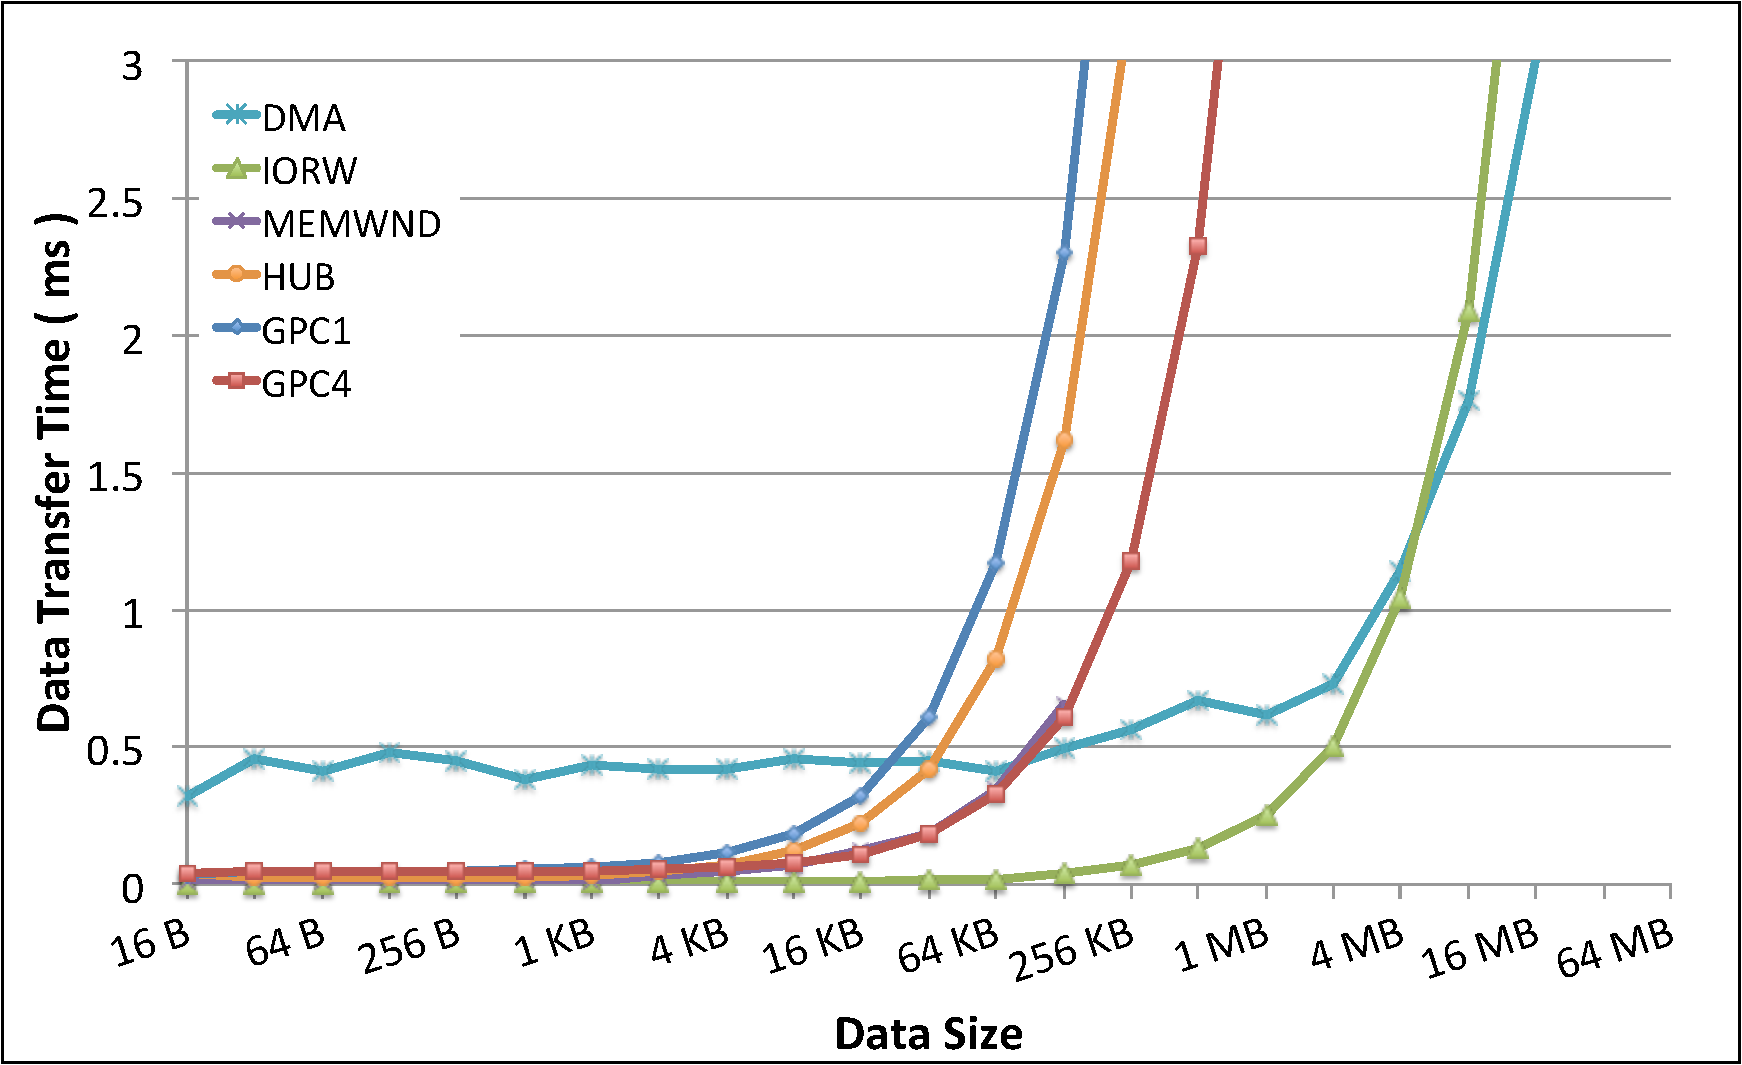
\includegraphics[width=0.34\textwidth]{figure/Graph/realtask/Memcpy_rtask_memswap_HtoD.pdf}}\\
  \subfigure[Device to Host]{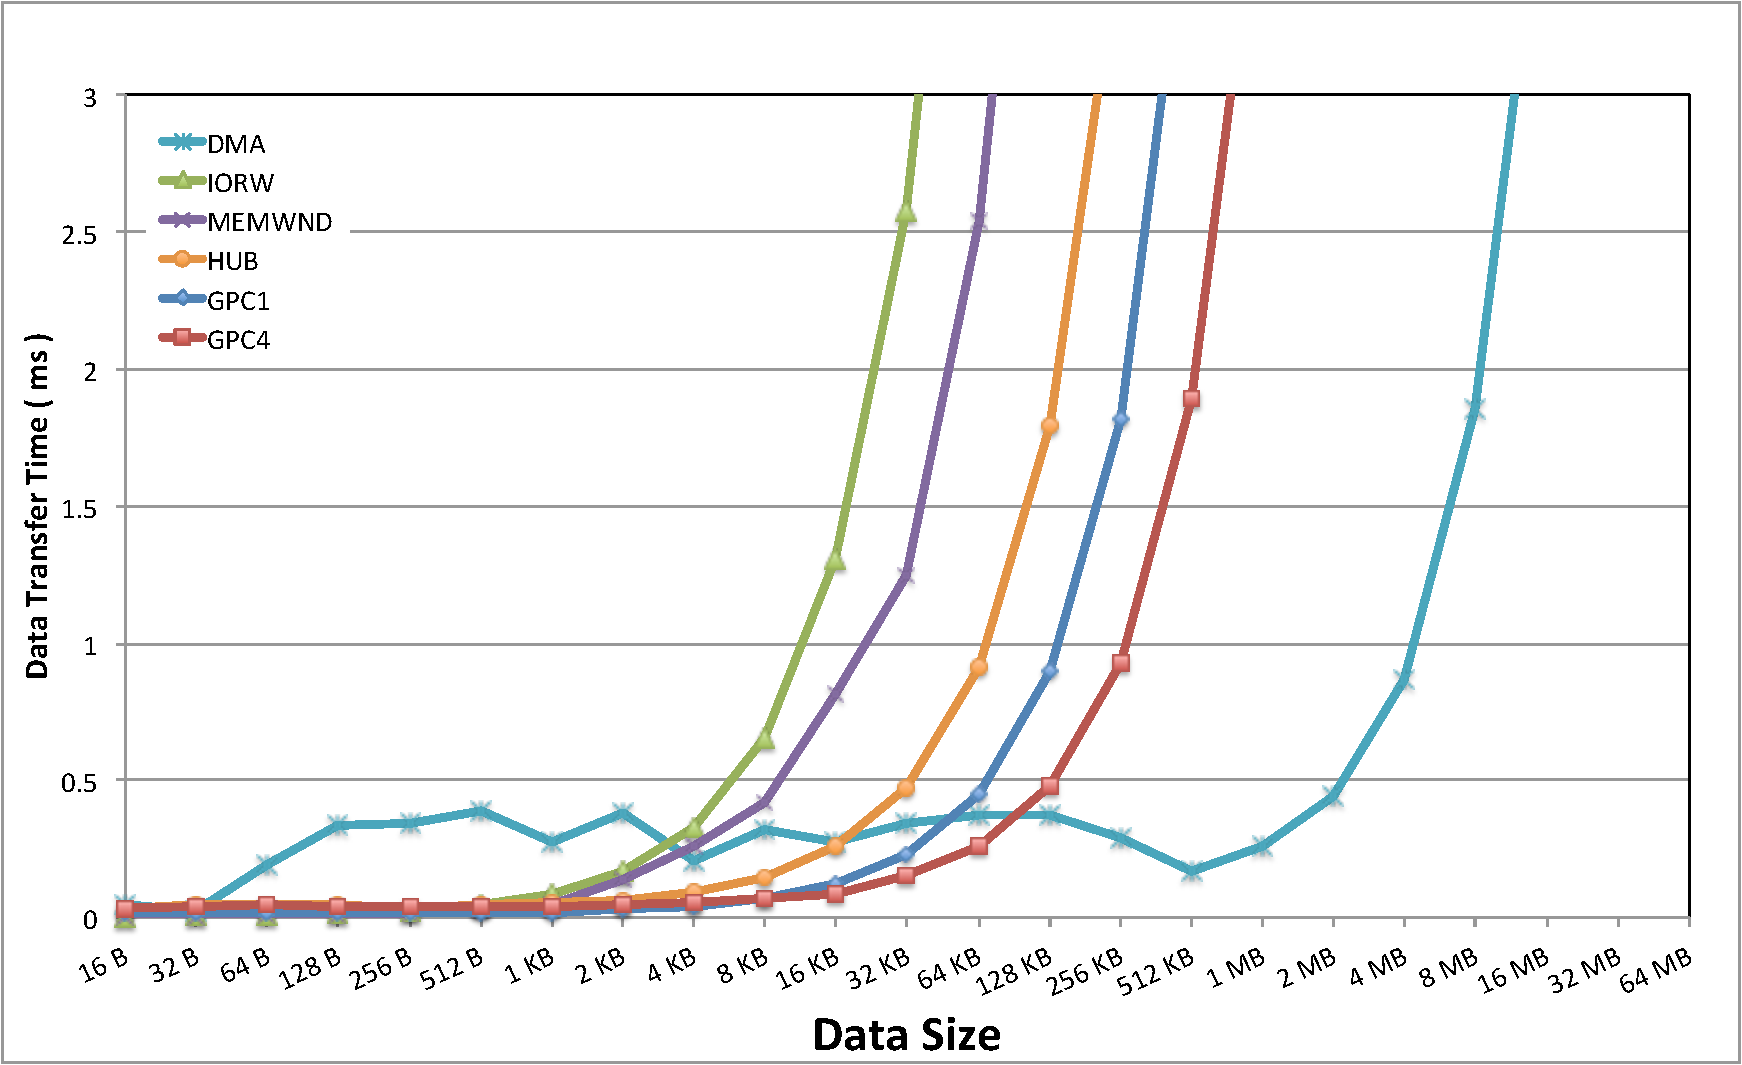
\includegraphics[width=0.34\textwidth]{figure/Graph/realtask/Memcpy_rtask_memswap_DtoH.pdf}}
  \caption{Average performance of each data transfer method with a
  real-time task under high memory pressure.}
  \label{fig:average_realtime_memswap}
 \end{center}
\end{figure}
\begin{figure}[!t]
 \begin{center}
  \subfigure[Host to Device]{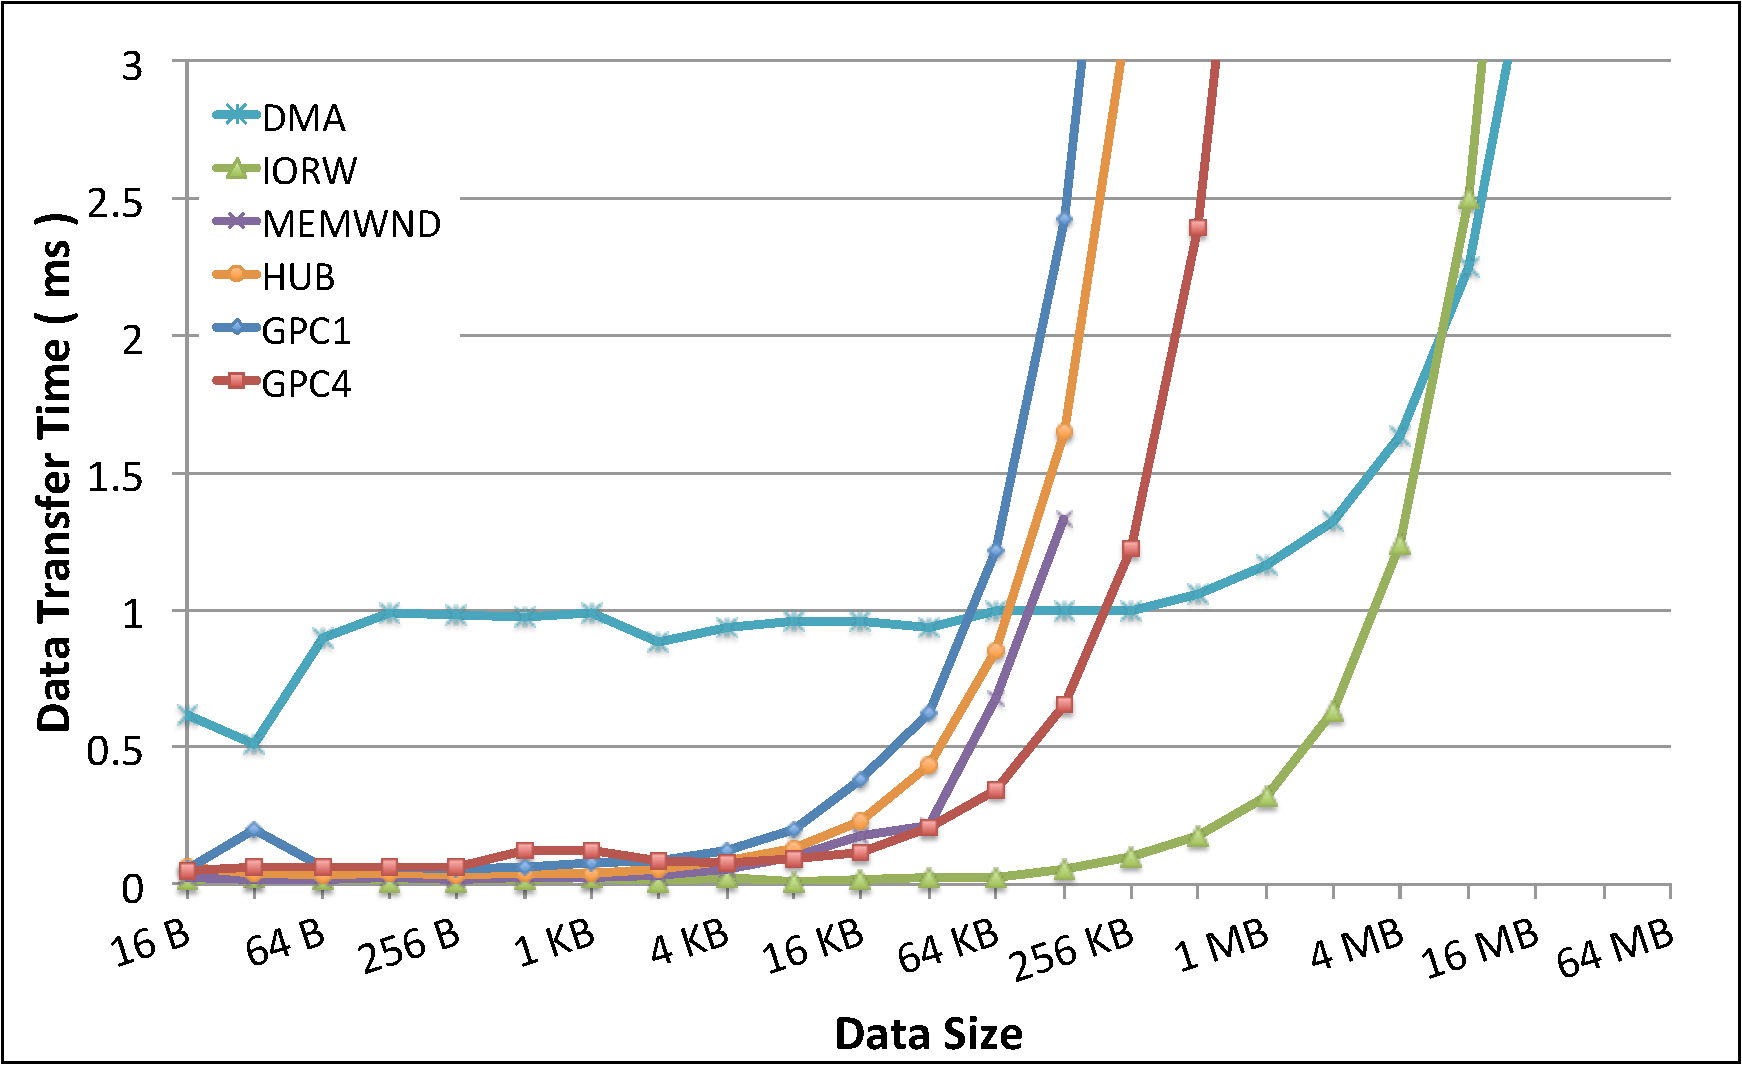
\includegraphics[width=0.34\textwidth]{figure/Graph/realtask/Memcpy_rtask_memswap_HtoD_worst.pdf}}\\
  \subfigure[Device to Host]{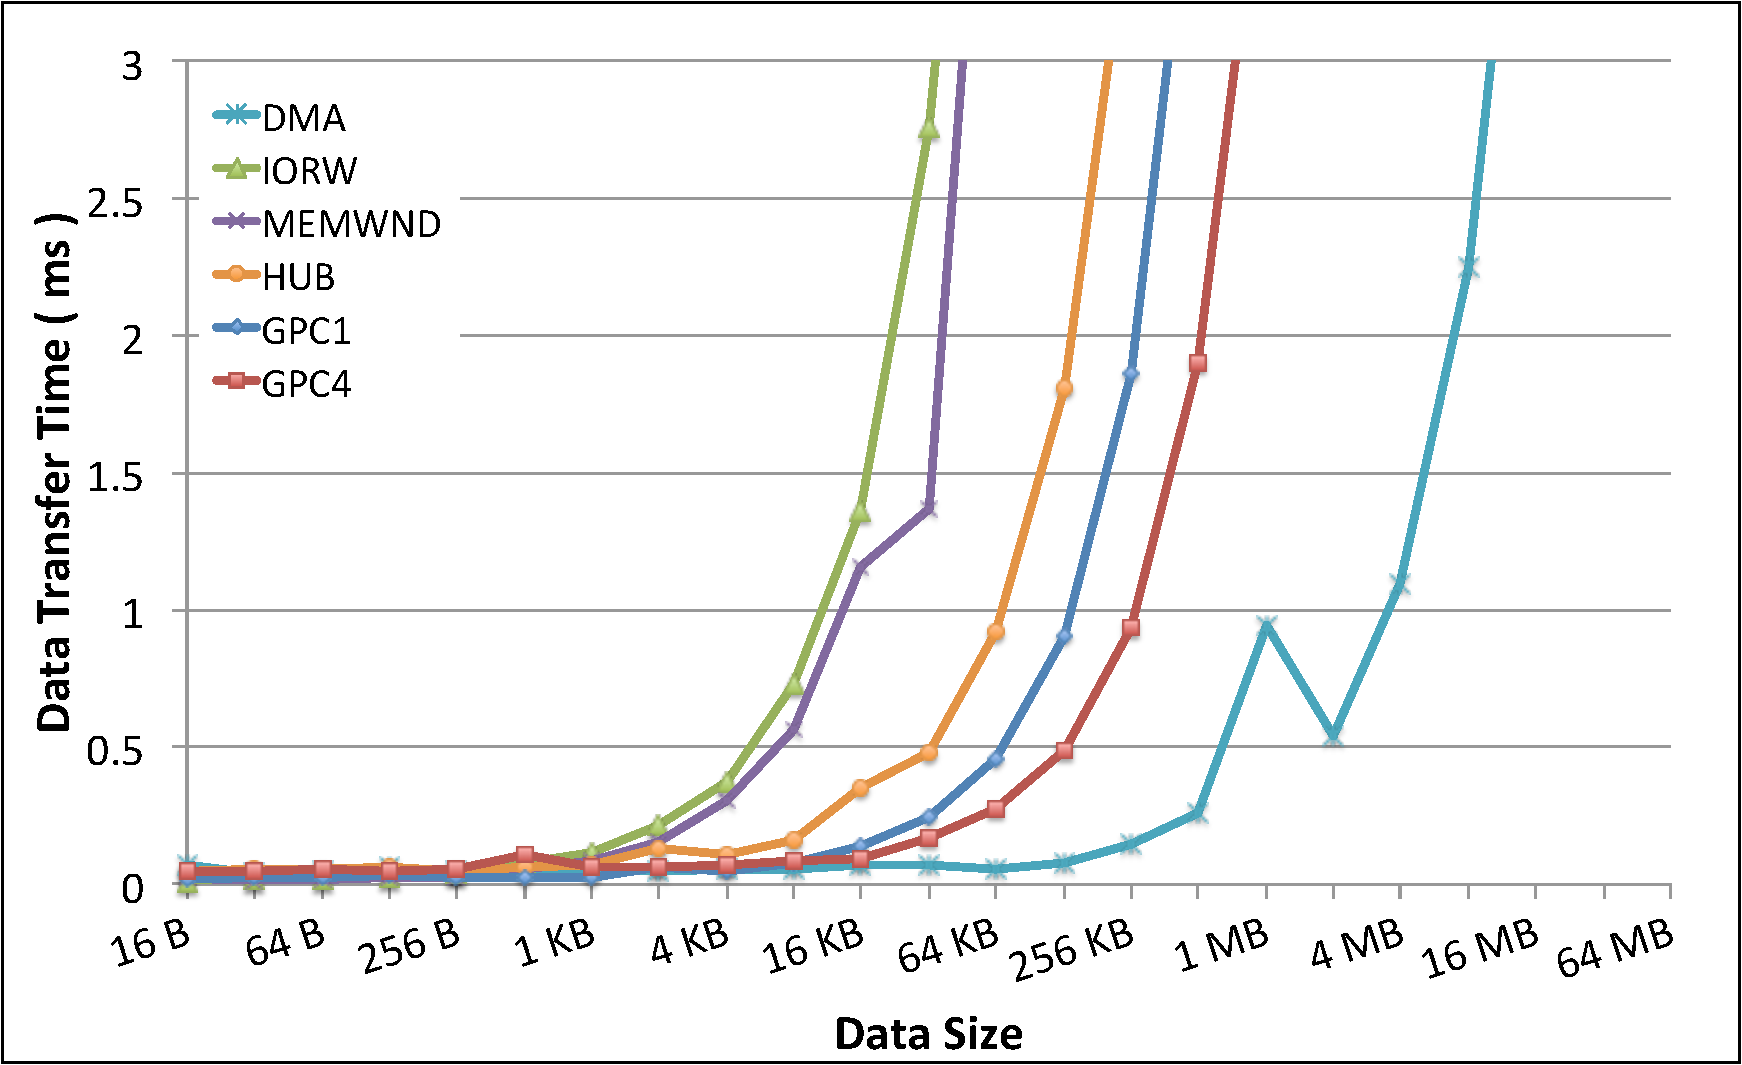
\includegraphics[width=0.34\textwidth]{figure/Graph/realtask/Memcpy_rtask_memswap_DtoH_worst.pdf}}
  \caption{Worst-case performance of each data transfer method with a
  real-time task under high memory pressure.}
  \label{fig:worst_realtime_memswap}
 \end{center}
\end{figure}

From now on, we restrict our attention to a real-time task.
We next evaluate the performance of each data transfer method under high
memory pressure, creating another task that eats up host memory space.
In some sense, this is not a meaningful experiment because we use the
pinned host memory space to allocate buffers while the memory pressure
is supposed to compel the paged host memory space.
Having said that, the memory pressure could still impose indirect
interference on real-time tasks~\cite{Kato_RTSJ11, Yang_OSDI08}.
It is worth conducting this experiment.
As demonstrated in
Figure~\ref{fig:average_realtime_memswap}~and~\ref{fig:worst_realtime_memswap},
the impact of memory pressure on the data transfer performance is
negligible.
This means that all the data transfer methods investigated in this paper
require not much paged host memory space.
Otherwise they must be interfered by memory workload.

\begin{figure}[!t]
 \begin{center}
  \subfigure[Host to Device]{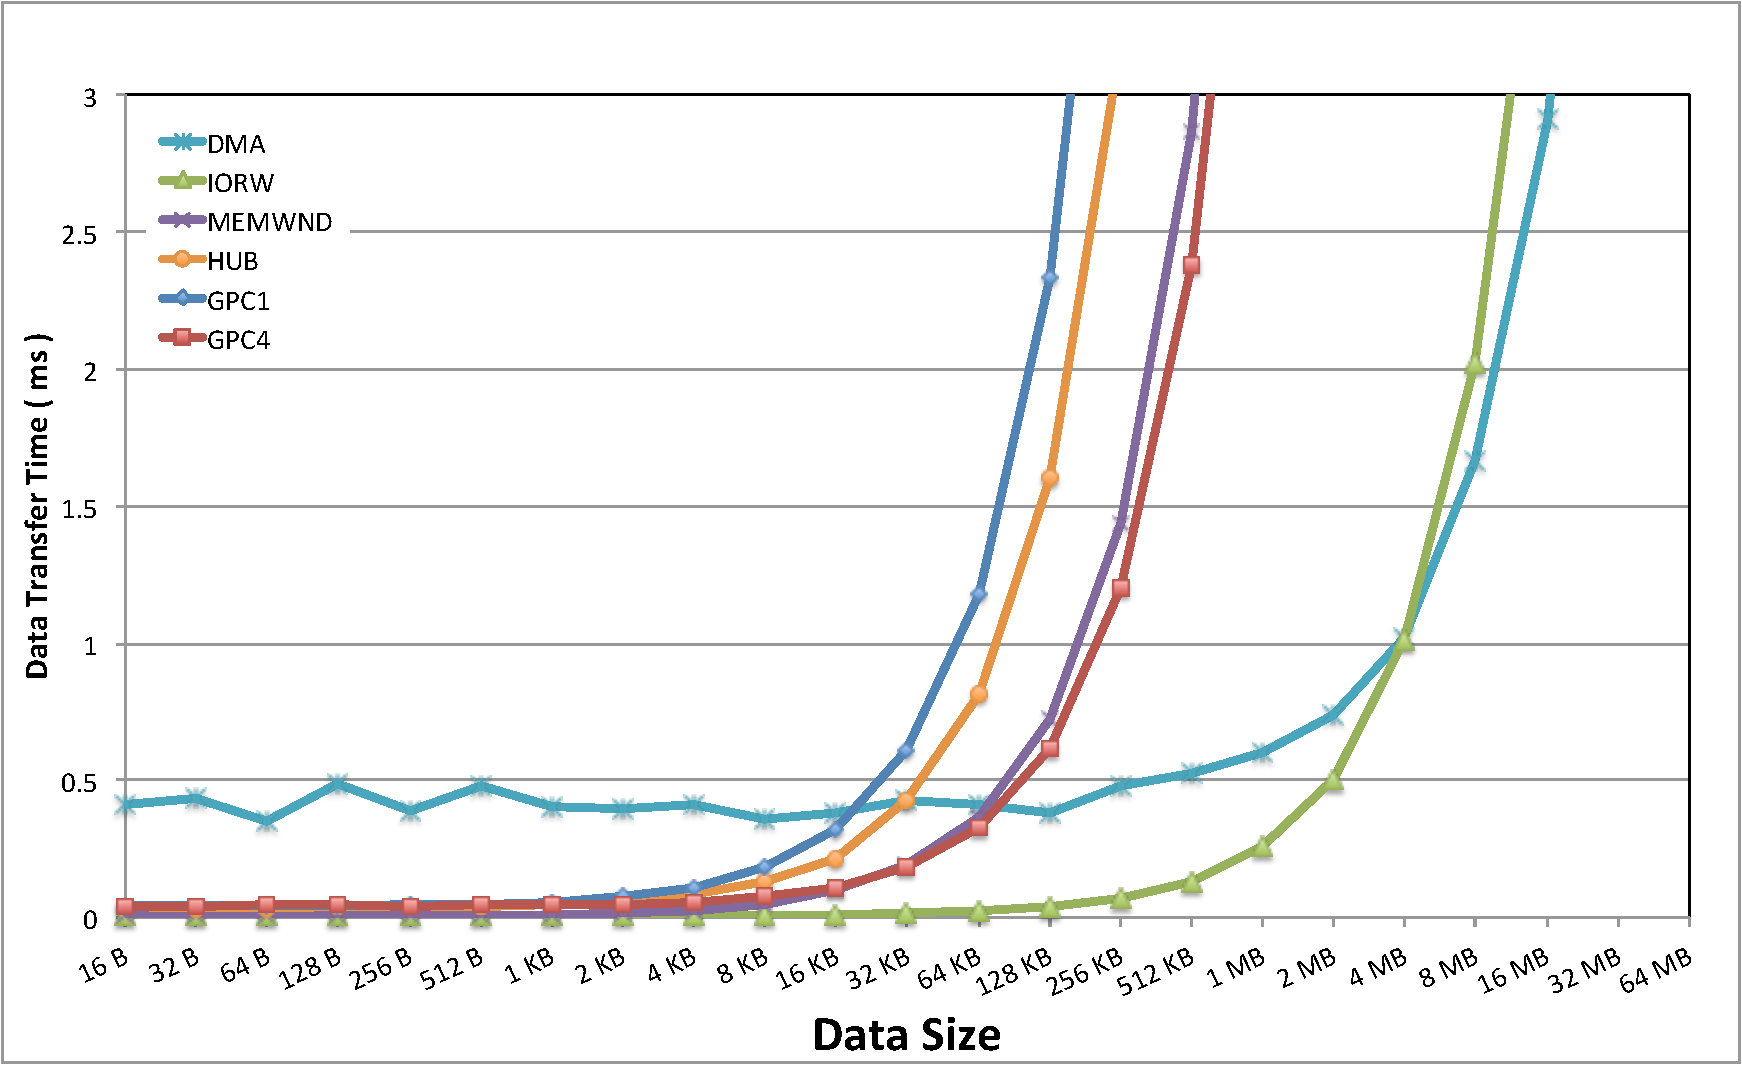
\includegraphics[width=0.34\textwidth]{figure/Graph/realtask/Memcpy_rtask_hackbench_HtoD.pdf}}\\
  \subfigure[Device to Host]{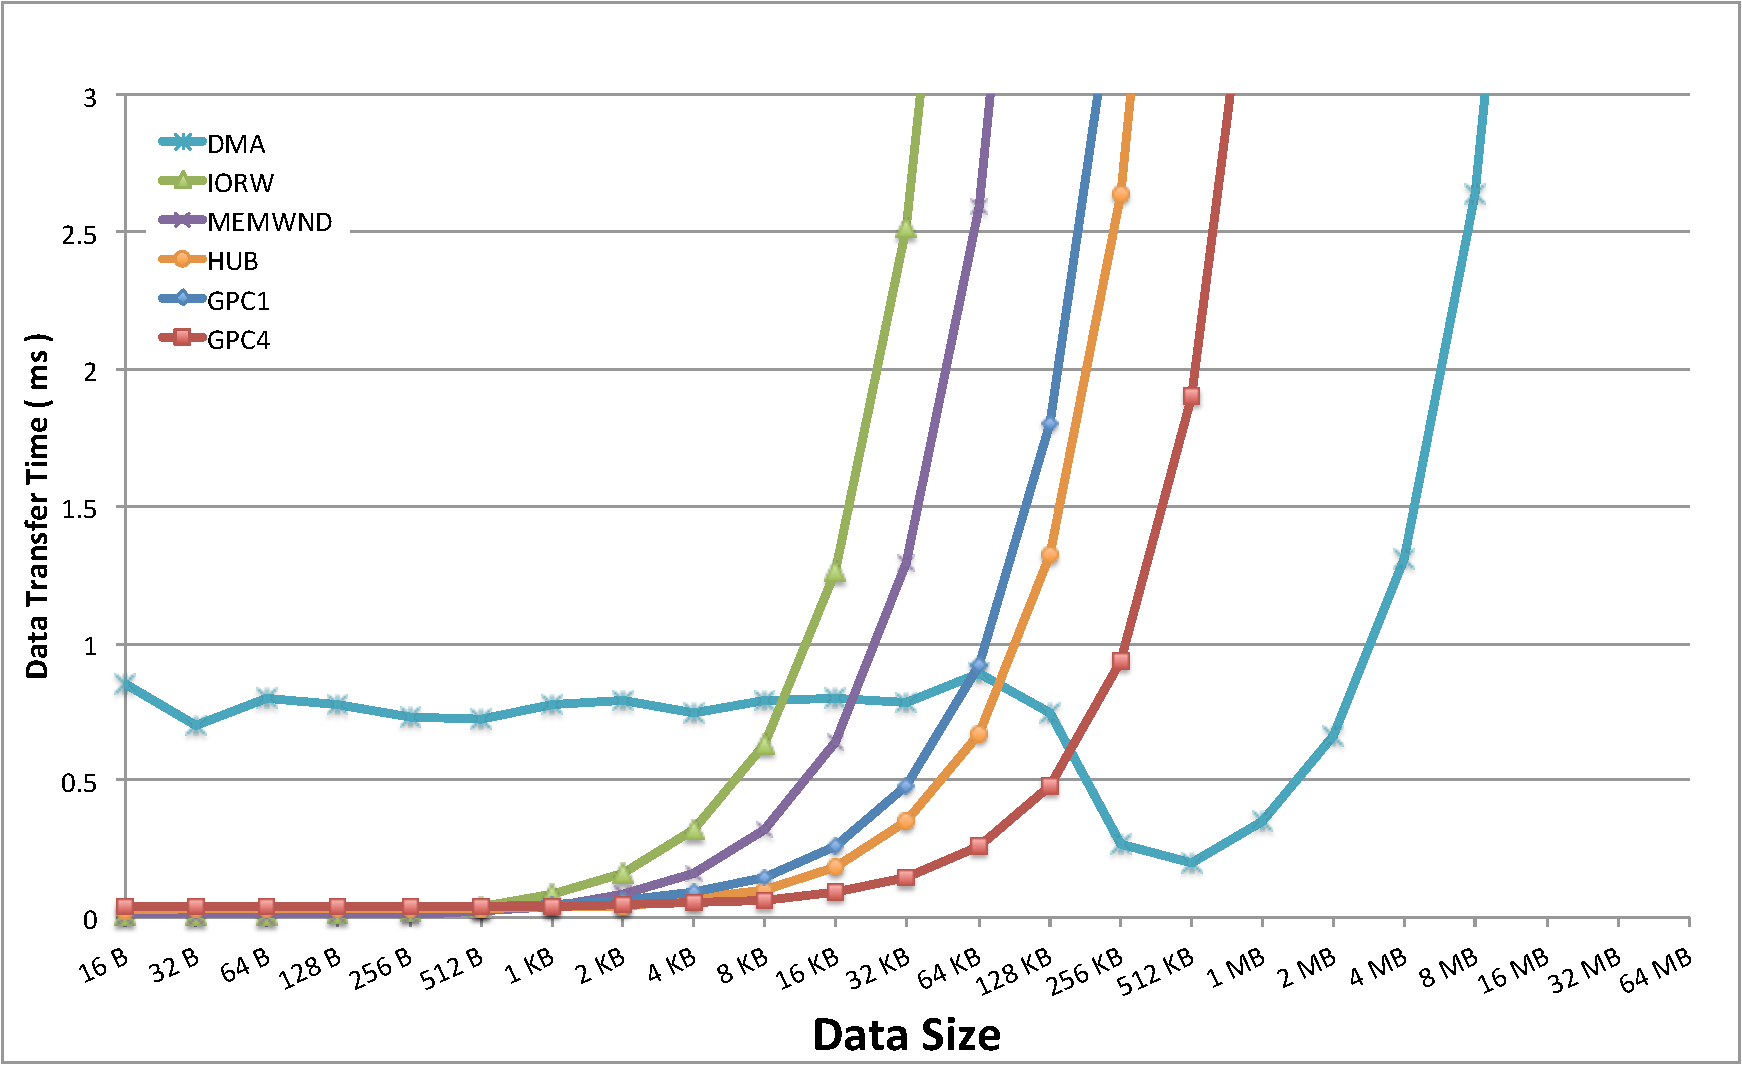
\includegraphics[width=0.34\textwidth]{figure/Graph/realtask/Memcpy_rtask_hackbench_DtoH.pdf}}
  \caption{Average performance of each data transfer method with a
  real-time task in the presence of \textsf{hackbench}.}
  \label{fig:average_realtime_hackbench}
 \end{center}
\end{figure}
\begin{figure}[!t]
 \begin{center}
  \subfigure[Host to Device]{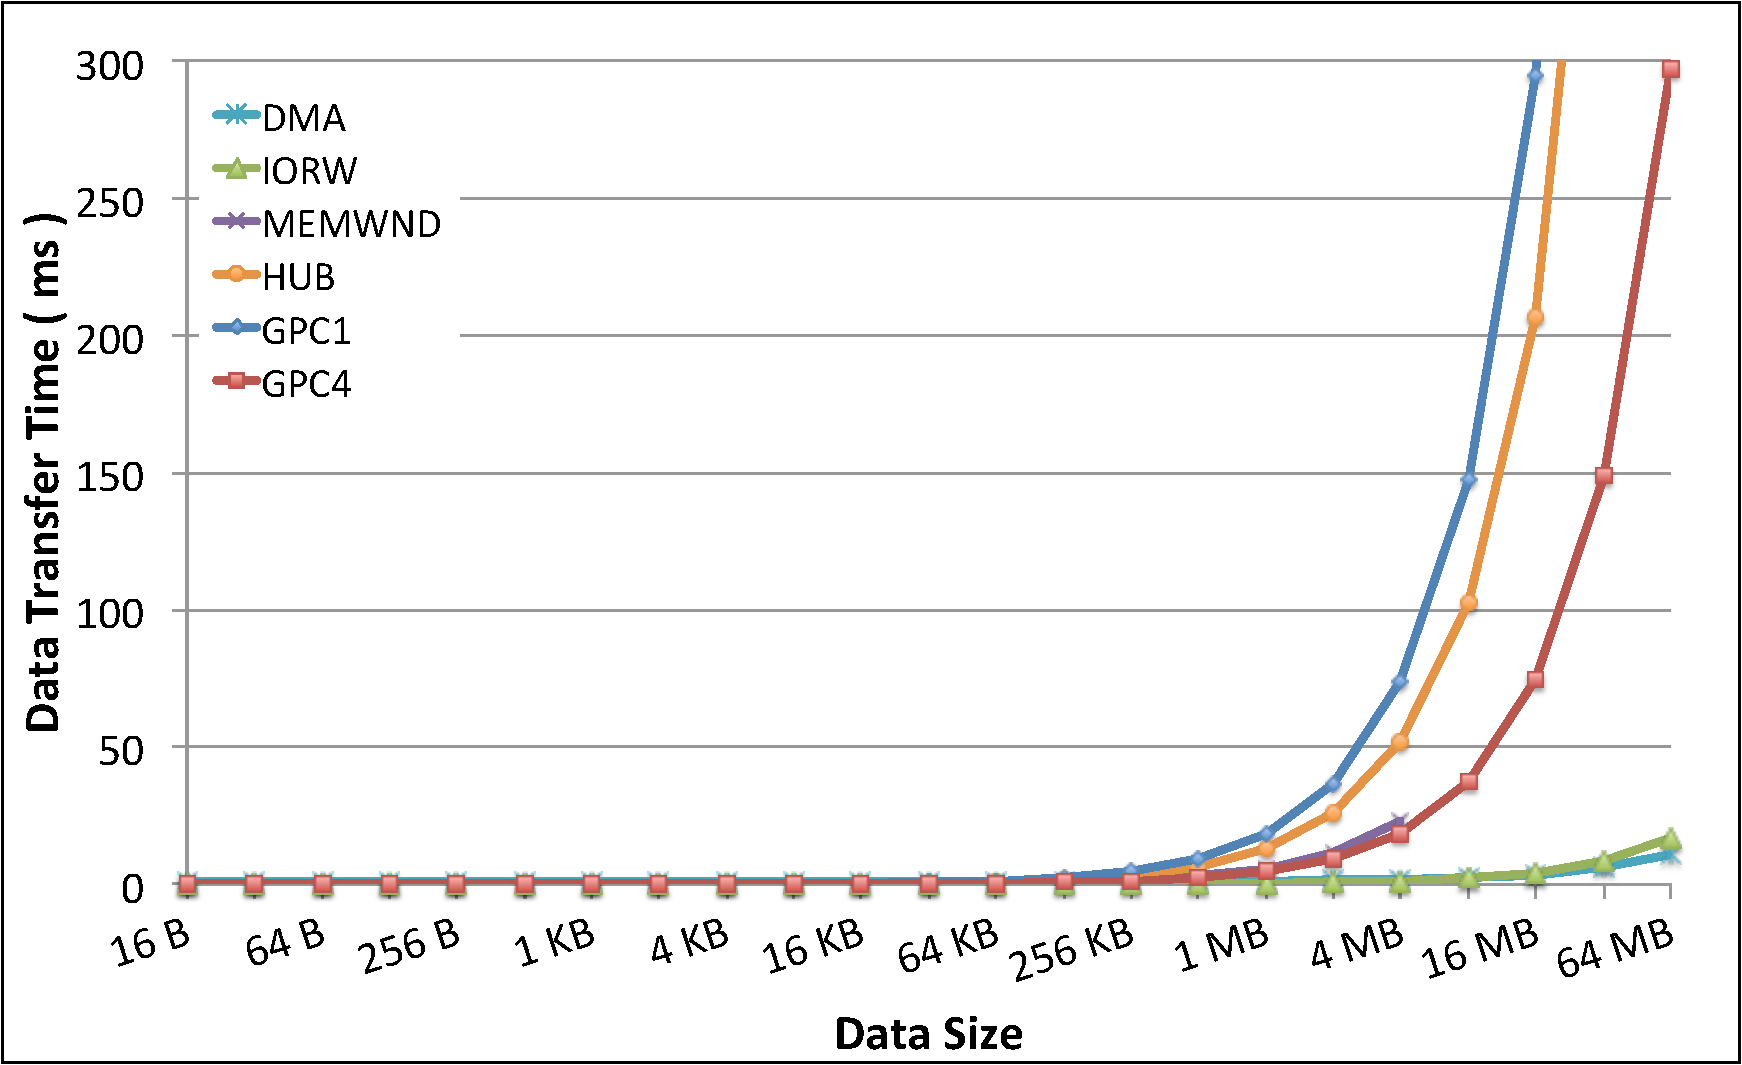
\includegraphics[width=0.34\textwidth]{figure/Graph/realtask/Memcpy_rtask_hackbench_HtoD_worst.pdf}}\\
  \subfigure[Device to Host]{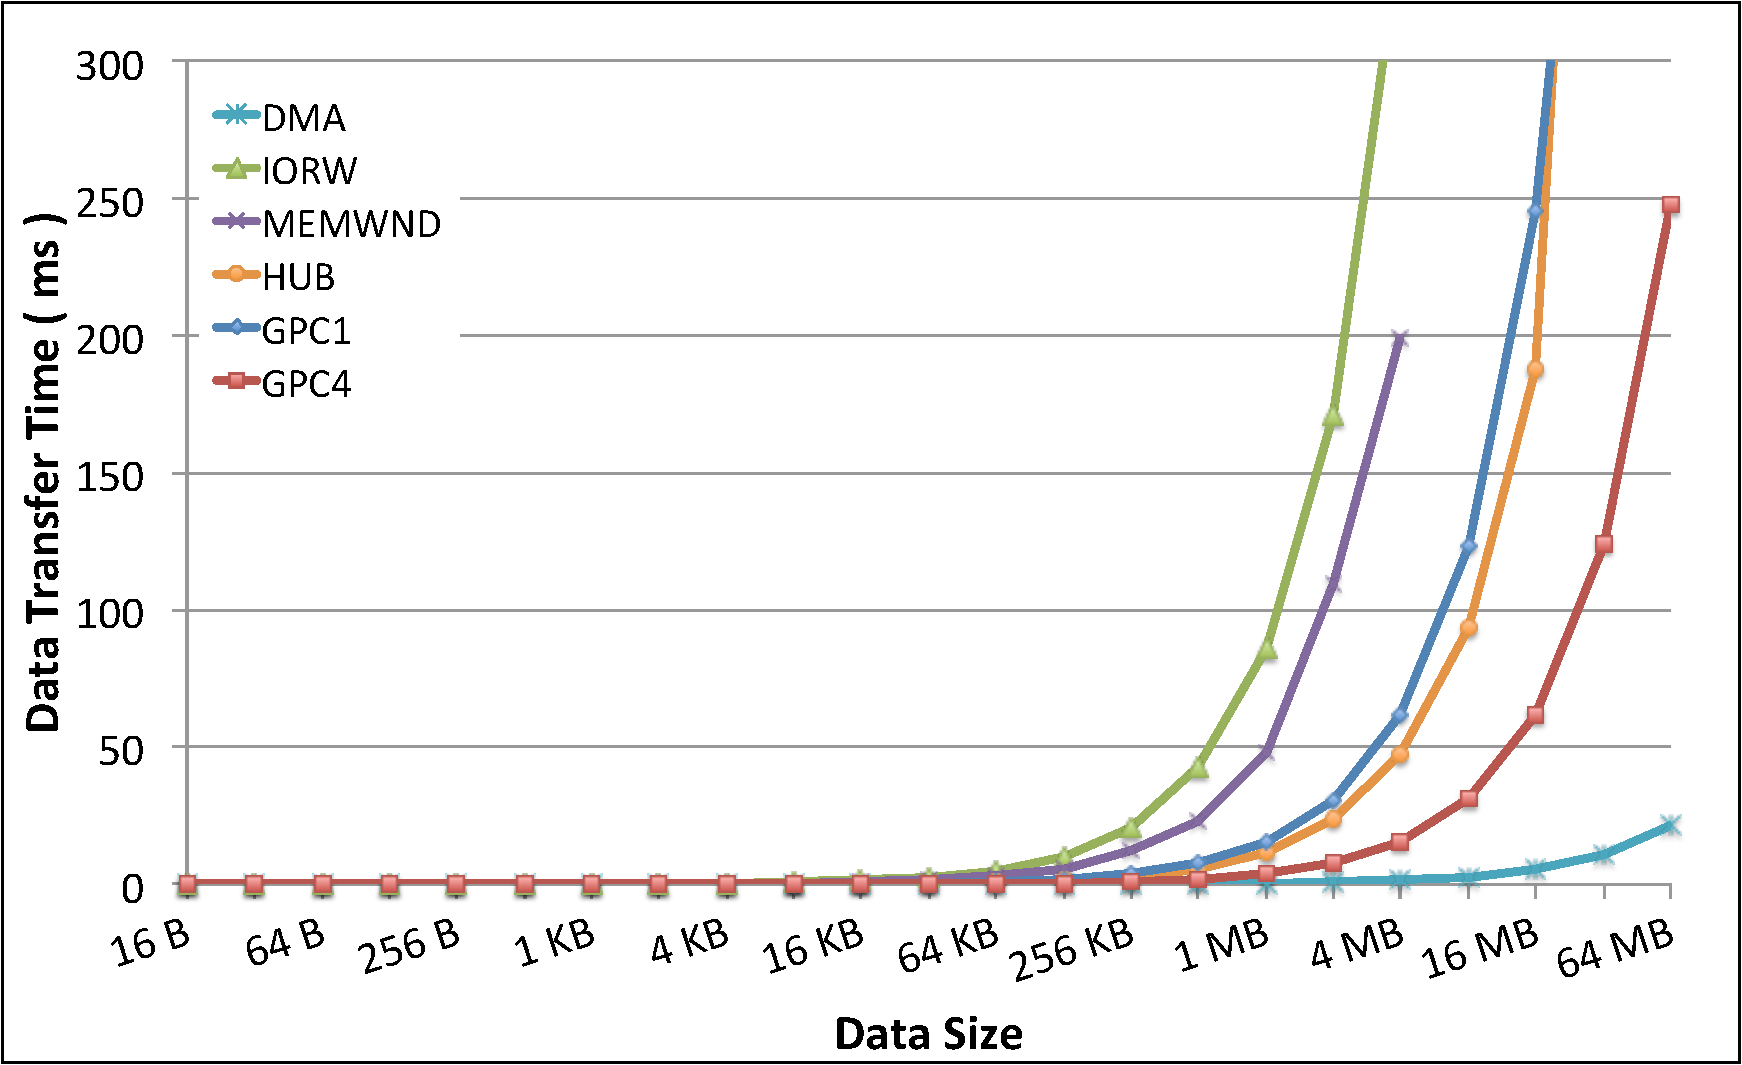
\includegraphics[width=0.34\textwidth]{figure/Graph/realtask/Memcpy_rtask_hackbench_DtoH_worst.pdf}}
  \caption{Worst-case performance of each data transfer method with a
  real-time task in the presence of \textsf{hackbench}.}
  \label{fig:worst_realtime_hackbench}
 \end{center}
\end{figure}

Figure~\ref{fig:average_realtime_hackbench}~and~\ref{fig:worst_realtime_hackbench}
show the average and the worst-case performance of each data transfer
method respectively, when a misbehaving \textsf{hackbench} process coexists.
\textsf{hackbench} is a tool that generates many processes executing I/O
system calls with pipes.
The results are all similar to the previous ones.
Since the Linux real-time scheduler is now well enhanced to protect a
real-time task from such misbehaving workload, these results are obvious
and trivial in some sense, but we can lead to a conclusion from a series
of the above experiments that \textit{the data transfer methods for the
GPU can be protected by the traditional real-time scheduler capability}.
This is a useful finding to facilitate an integration of real-time
systems and GPU computing.

\subsection{Concurrent Performance}

\begin{figure}[!t]
 \begin{center}
  \subfigure[Host to Device]{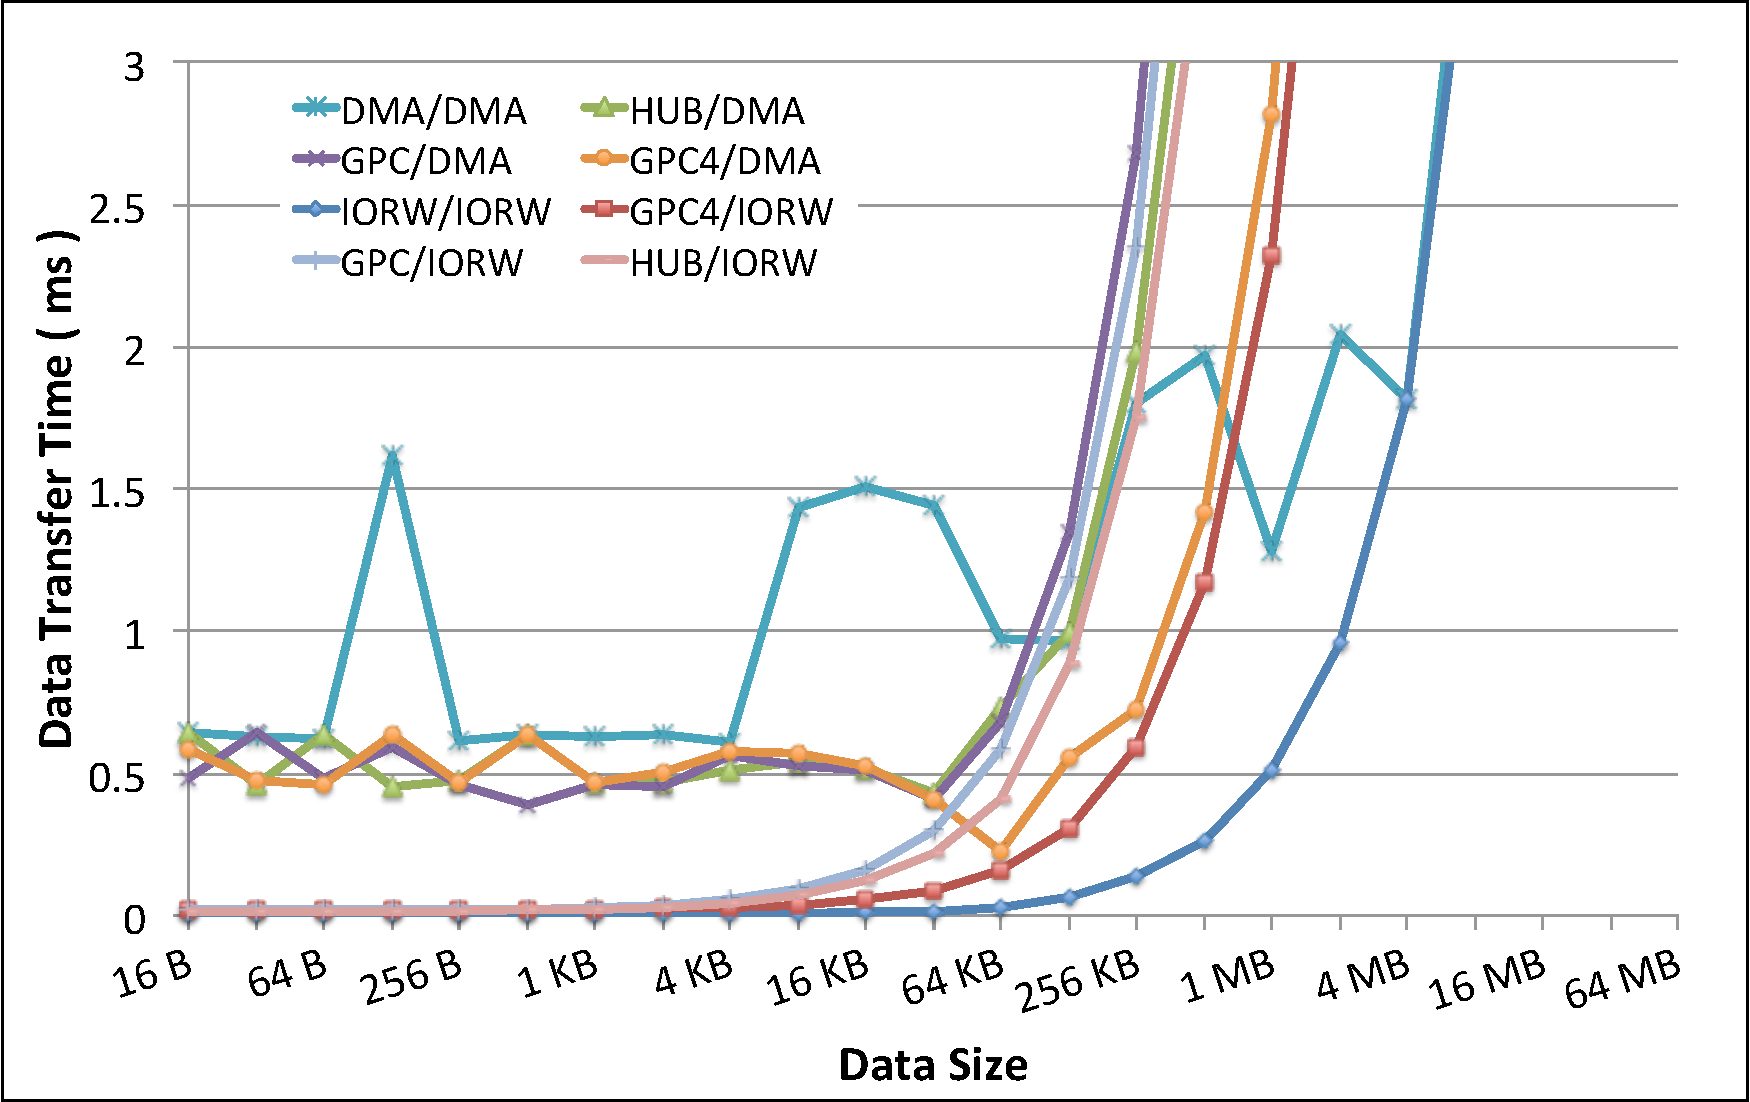
\includegraphics[width=0.34\textwidth]{figure/Graph/not_realtask/Memcpy_hybrid_HtoD.pdf}}\\
  \subfigure[Device to Host]{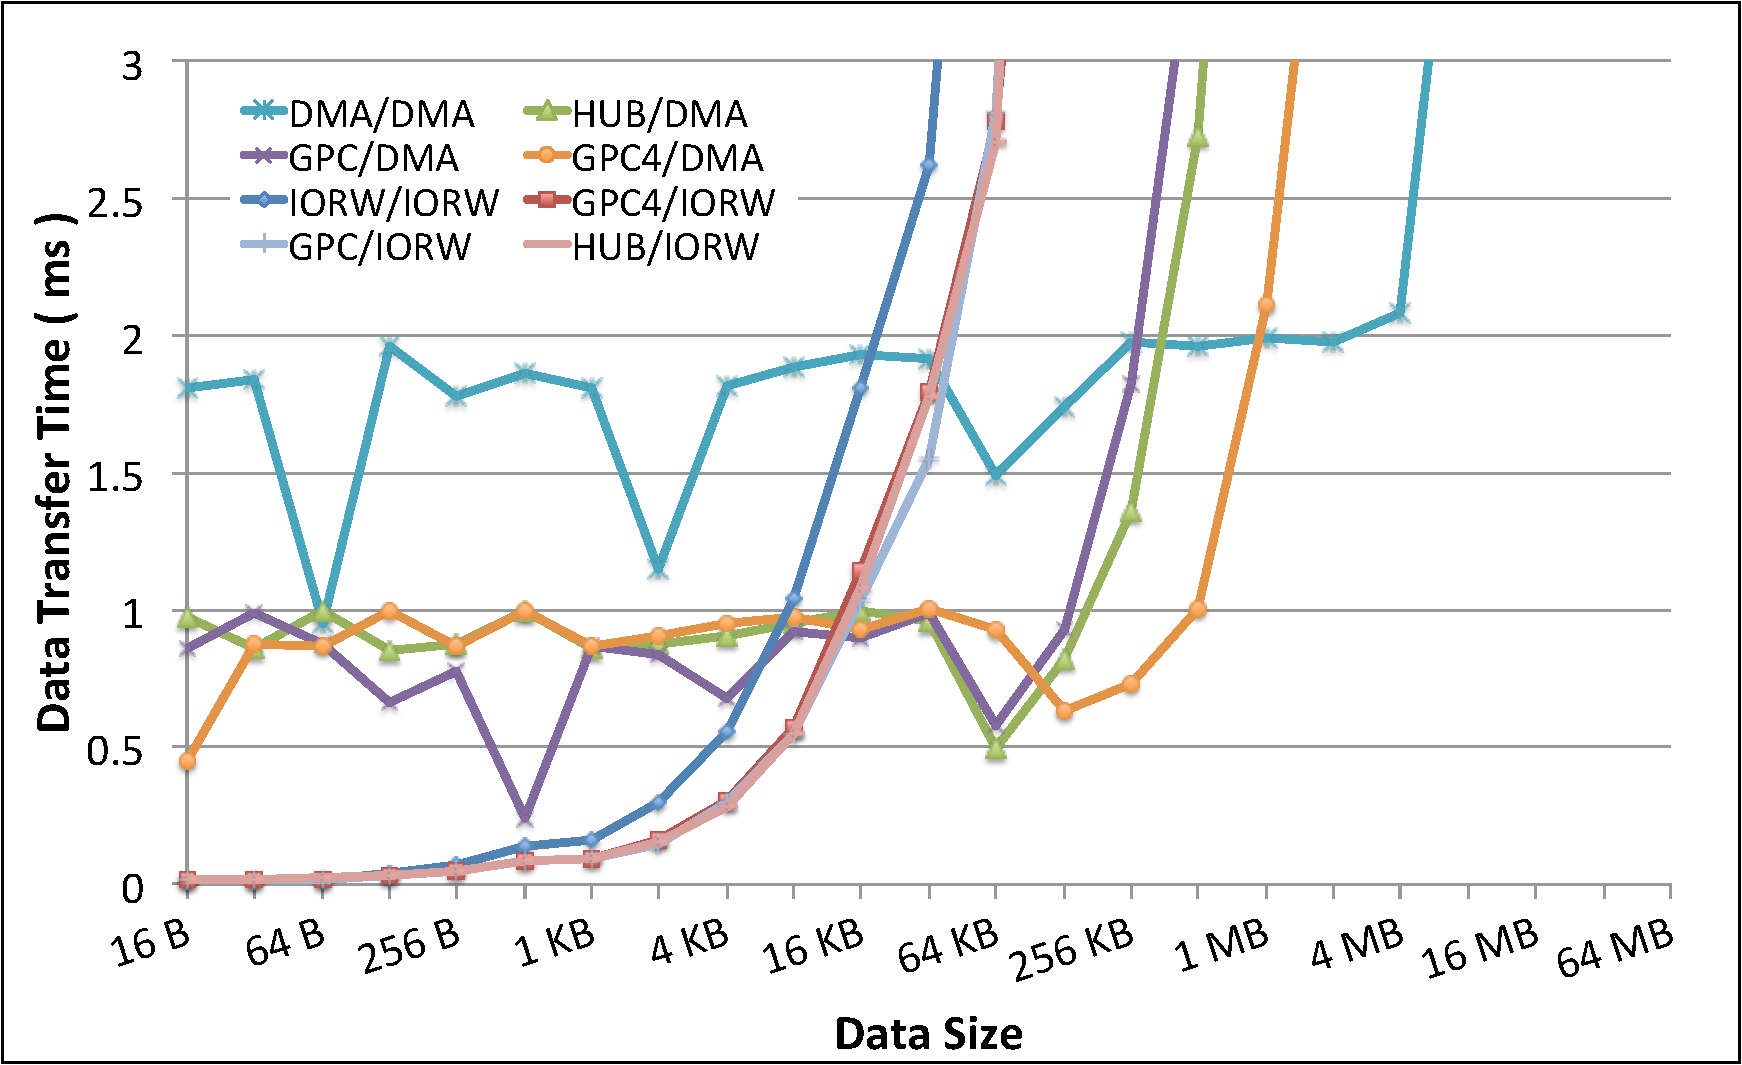
\includegraphics[width=0.34\textwidth]{figure/Graph/not_realtask/Memcpy_hybrid_DtoH.pdf}}\\
  \caption{Average performance of combinations of the data transfer
  methods for concurrent real-time tasks.}
  \label{fig:average_realtime_concurrent}
 \end{center}
\end{figure}
\begin{figure}[!t]
 \begin{center}
  \subfigure[Host to Device]{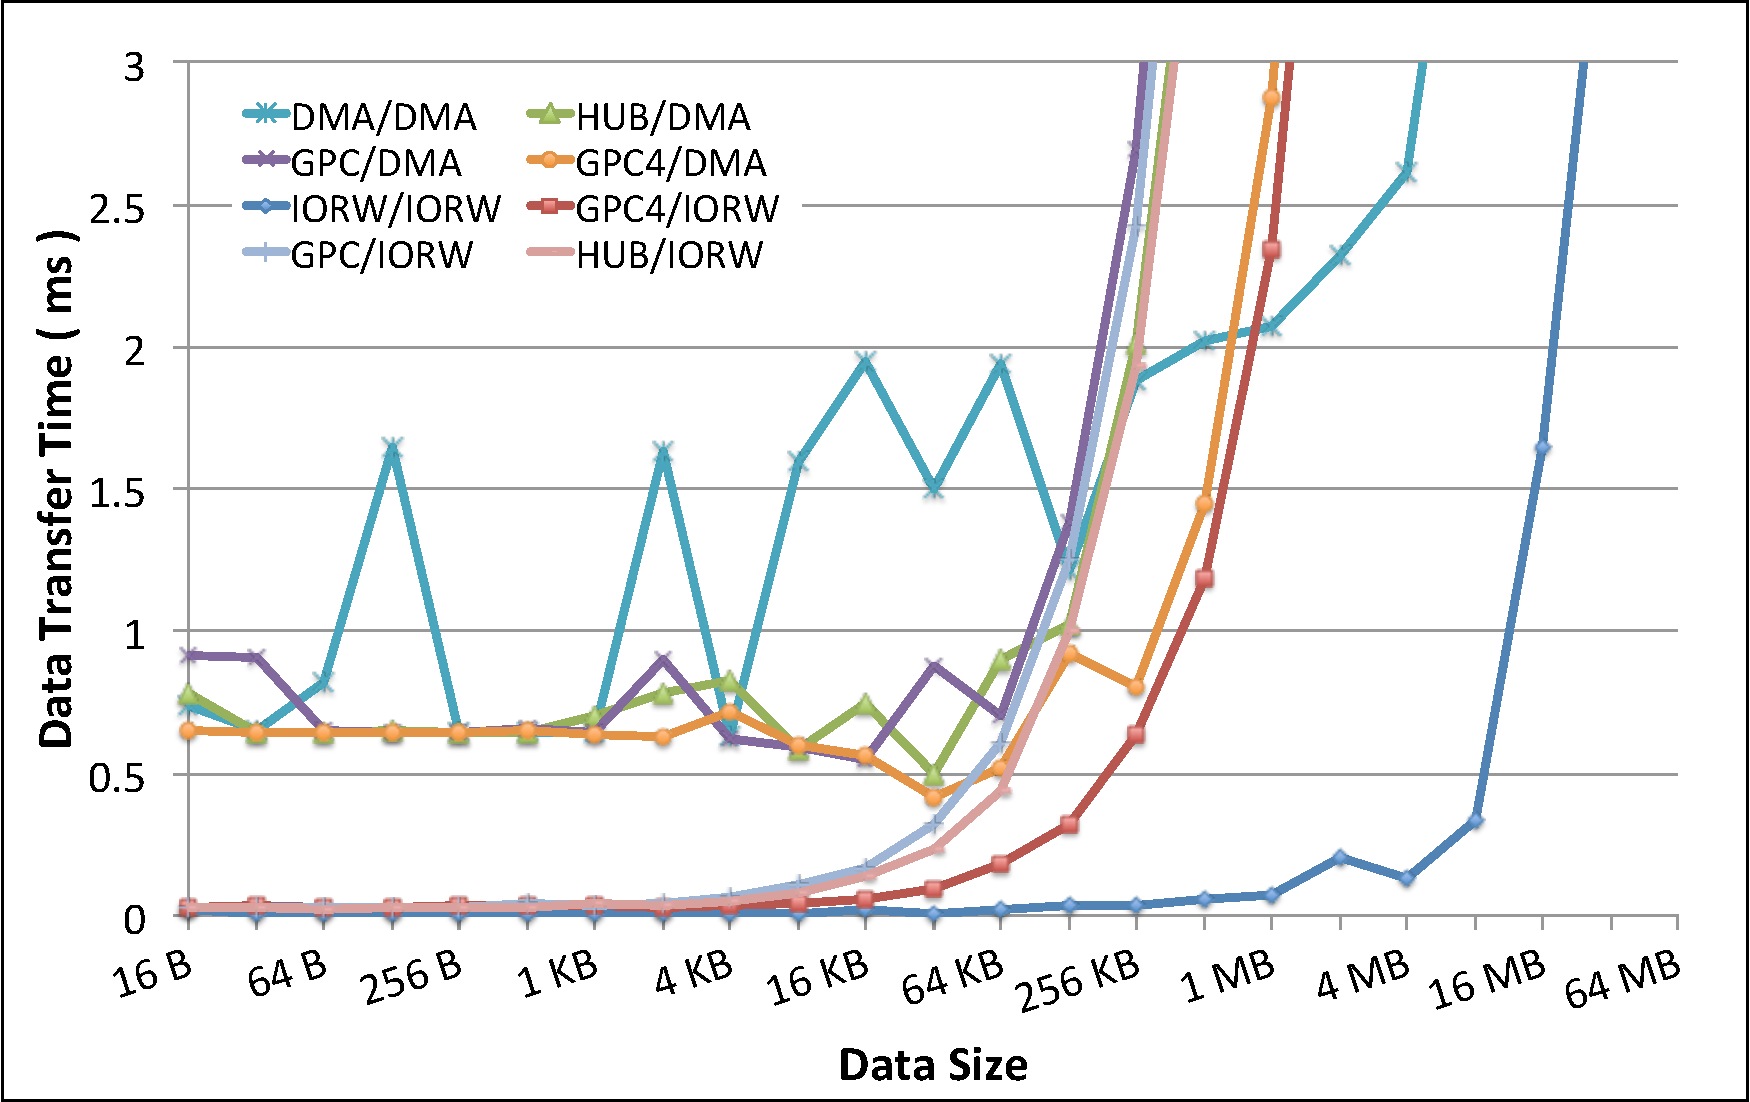
\includegraphics[width=0.34\textwidth]{figure/Graph/not_realtask/Memcpy_hybrid_HtoD_worst.pdf}}\\
  \subfigure[Device to Host]{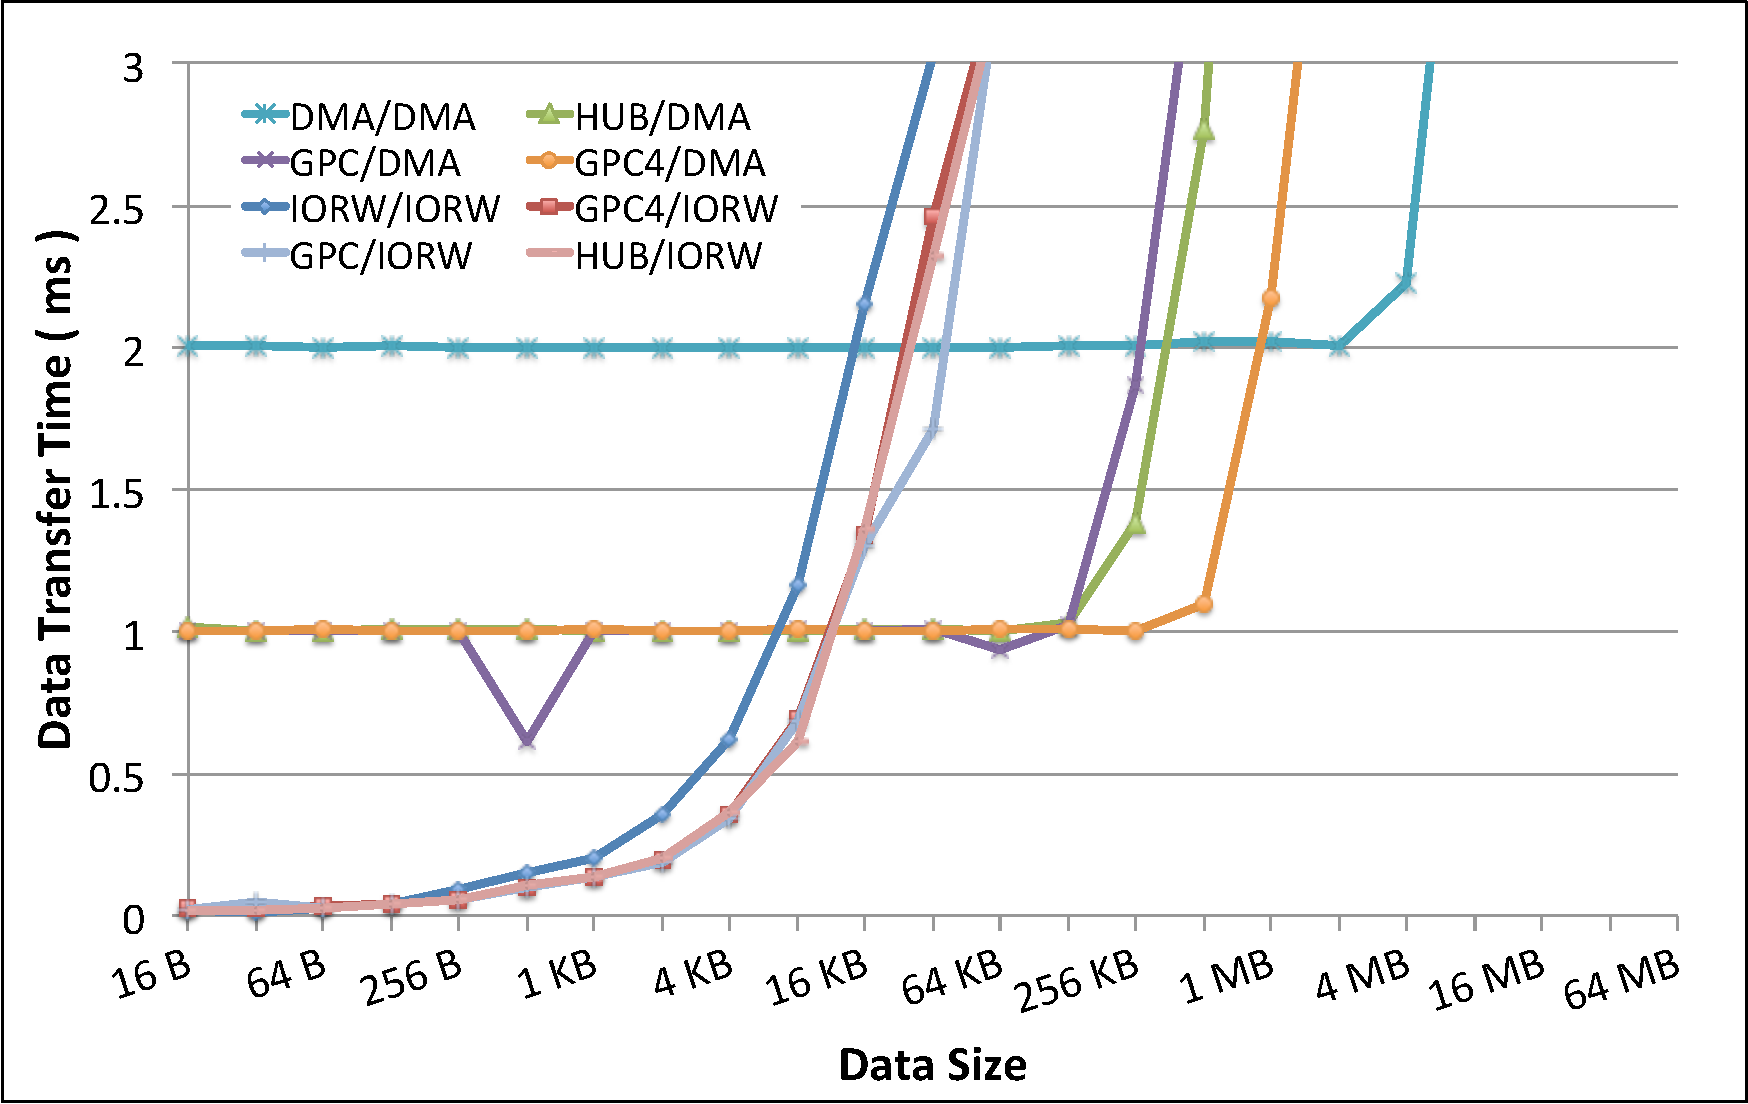
\includegraphics[width=0.34\textwidth]{figure/Graph/not_realtask/Memcpy_hybrid_DtoH_worst.pdf}}\\
  \caption{Worst-case performance of combinations of the data transfer
  methods for concurrent real-time tasks.}
  \label{fig:worst_realtime_concurrent}
 \end{center}
\end{figure}

So far we have studied the capabilities of the investigated data
transfer methods and their causal relation to a real-time task.
We now evaluate the performance of concurrent \textit{two} data streams
using different combinations of the data transfer methods as shown in
Figure~\ref{fig:average_realtime_concurrent}~and~\ref{fig:worst_realtime_concurrent}.
This is a very interesting result.
For the host-to-device direction, the best performance is obtained when
both the two tasks use \textsf{IORW}.
In this case, the two data streams are not overlapped but are processed
in sequential due to the use of the same \textsf{IORW} path.
Nonetheless it outperforms the other combinations because the
performance of \textsf{IORW} is way higher than the other methods as we
have observed in a series of the previous experiments.
However, the device-to-host direction shows a different performance.
Since \textsf{IORW} becomes slow when the CPU reads the device memory as
mentioned in Section~\ref{sec:basic_performance},
\textsf{IORW}/\textsf{IORW} is not the best performer any longer.
Instead using the microcontroller(s) provides the best performance until
$2$MB.
This is attributed to the fact that the microcontroller-based data
transfer method can be overlapped with any other data transfer methods.
From $16$B to $16$KB, a combination of the microcontroller and
\textsf{IORW} is the fastest, while that of the microcontroller and
\textsf{DMA} is the fastest from $16$KB to $2$MB.
Note that from $16$B to $16$KB the performance is aligned with the slow
\textsf{IORW} curve.
Therefore the choice of \textsf{HUB}, \textsf{GPC}, and \textsf{GPC4}
does not really matter to the performance.
However, from $16$KB to $2$MB the performance is improved by using four
microcontrollers in parallel (\textit{i.e.}, \textsf{GPC4}), since
\textsf{DMA} is faster than the microcontroller and
thereby the performance is aligned with the microcontroller curve.
We learn from this experiment that the microcontroller is useful to
overlap concurrent data streams with \textsf{DMA} or \textsf{IORW}, and
using multiple microcontrollers in parallel can further improve the
performance of concurrent data transfers.


\section{Conclusion}
\label{sec:conclusion}

In this paper, we have presented an investigation and empirical
comparison of the data transfer methods for GPU computing.
We found that the hardware-based DMA and the I/O read and write methods
are the most effective to maximize the data transfer performance for a
single stream even in the presence of competing CPU workload.
On the other hand, the microcontroller-based method is useful to overlap
the data transfer with the DMA or the IO read and write methods,
reducing the total makespan of multiple data streams.
We also demonstrated that the traditional real-time CPU scheduler can
shield the data transfer of a real-time task from performance
interference.
We believe that all these findings are useful contributions to develop
an integration of real-time systems and GPU computing.

Our open-source implementations of the data transfer methods
provided in this paper may be downloaded from
\url{http://github.com/shinpei0208/gdev/}.

In future work, we will investigate how to optimize the choice of data
transfer methods depending on the target system and workload.
Since user programs use the same API function for the data transfer, the
underlying system software must understand environments and choose
appropriate data transfer methods to maximize the performance and/or
miminize the latency.
Runtime management of soft real-time capabilities of GPU computing is
also a core challenge for future work.

\bibliographystyle{plain}
{\footnotesize
\bibliography{references}
}

\end{document}



